% =====================================================================
%  MCMP117 -- Fundamentals of Operating Systems
%  Week 7 Course Notes: Virtual Memory & File Systems
%  Compile with XeLaTeX (twice):  xelatex MCMP117_Week7_Notes.tex
%  Needs ./figures/ and the ../code/ folder.
% =====================================================================
\documentclass[11pt,a4paper]{article}
\newcommand{\weeknum}{7}
% ---------- Page & fonts ---------------------------------------------
\usepackage[a4paper,margin=2.3cm,headheight=15pt]{geometry}
\usepackage{fontspec}
\IfFontExistsTF{Calibri}{\setmainfont{Calibri}}{\setmainfont{Carlito}}
\IfFontExistsTF{Cambria}{\newfontfamily\headfont{Cambria}}{\newfontfamily\headfont{Caladea}}
\IfFontExistsTF{Consolas}{\setmonofont[Scale=0.95]{Consolas}}{\setmonofont[Scale=0.88]{DejaVu Sans Mono}}
\usepackage{amsmath,amssymb}
\usepackage{microtype}
\linespread{1.12}
\setlength{\parskip}{0.55em}
\setlength{\parindent}{0pt}

% ---------- Colours (course design system) ----------------------------
\usepackage{xcolor}
\definecolor{dark}{HTML}{212121}
\definecolor{charcoal}{HTML}{36454F}
\definecolor{slate}{HTML}{50808E}
\definecolor{mint}{HTML}{02C39A}
\definecolor{mintdeep}{HTML}{028090}
\definecolor{light}{HTML}{F2F2F2}
\definecolor{muted}{HTML}{6B7679}

% ---------- Packages ---------------------------------------------------
\usepackage{graphicx}
\usepackage{float}
\usepackage{needspace}
\graphicspath{{figures/}}
\usepackage[font=small,labelfont={bf,color=mintdeep},justification=centering]{caption}
\usepackage{booktabs,longtable,array,tabularx}
\usepackage{enumitem}
\setlist{itemsep=0.25em,topsep=0.3em}
\usepackage{tikz}
\usetikzlibrary{arrows.meta,positioning,calc,shapes.geometric}
\usepackage{pgfplots}
\pgfplotsset{compat=1.17}
\usepackage[most]{tcolorbox}
\usepackage{titlesec}
\usepackage{fancyhdr}
\usepackage{xurl}
\usepackage[colorlinks=true,linkcolor=mintdeep,urlcolor=mintdeep,citecolor=mintdeep]{hyperref}

% ---------- Headings ----------------------------------------------------
\titleformat{\section}{\headfont\Large\bfseries\color{charcoal}}{\color{mint}\thesection}{0.7em}{}
\titleformat{\subsection}{\headfont\large\bfseries\color{charcoal}}{\color{mintdeep}\thesubsection}{0.6em}{}
\titleformat{\subsubsection}{\headfont\normalsize\bfseries\color{mintdeep}}{}{0em}{}
\titlespacing*{\section}{0pt}{1.6em}{0.6em}
\titlespacing*{\subsection}{0pt}{1.2em}{0.4em}

% ---------- Header / footer -----------------------------------------------
\pagestyle{fancy}
\fancyhf{}
\fancyhead[L]{\small\color{muted}MCMP117 --- Fundamentals of Operating Systems}
\fancyhead[R]{\small\color{muted}Week \weeknum{} Notes}
\fancyfoot[C]{\small\color{muted}\thepage}
\renewcommand{\headrulewidth}{0pt}

% ---------- Boxes ---------------------------------------------------------
\newtcolorbox{keyidea}[1][Key idea]{enhanced,breakable,colback=charcoal,colframe=charcoal,
  coltext=white,fonttitle=\headfont\bfseries\color{mint},title={#1},
  attach title to upper={\par\smallskip},boxrule=0pt,arc=3pt,left=10pt,right=10pt,top=8pt,bottom=8pt}
\newtcolorbox{example}[1][Worked example]{enhanced,colback=light,colframe=light,
  fonttitle=\headfont\bfseries\color{mintdeep},title={#1},attach title to upper={\par\smallskip},
  boxrule=0pt,arc=3pt,left=10pt,right=10pt,top=8pt,bottom=8pt}
\newtcolorbox{tryit}[1][Try it yourself]{enhanced,breakable,colback=white,colframe=mint,
  fonttitle=\headfont\bfseries\color{mintdeep},title={#1},attach title to upper={\par\smallskip},
  boxrule=0.8pt,arc=3pt,left=10pt,right=10pt,top=8pt,bottom=8pt}
\newtcolorbox{histnote}[1][Historical note]{enhanced,breakable,colback=white,colframe=slate!40,
  fonttitle=\headfont\bfseries\color{slate},title={#1},attach title to upper={\par\smallskip},
  boxrule=0.5pt,arc=3pt,left=10pt,right=10pt,top=8pt,bottom=8pt,fontupper=\small}

% Photo helper: fits image inside a box, never distorted (keepaspectratio)
\newcommand{\photo}[3]{\includegraphics[width=#1,height=#2,keepaspectratio]{#3}}

\newcommand{\term}[1]{\textbf{\color{mintdeep}#1}}
\newcommand{\cmd}[1]{\texttt{#1}}


% ---------- Code listings ----------------------------------------------------
\usepackage{listings}
\lstdefinestyle{course}{
  basicstyle=\ttfamily\small, columns=fullflexible, keepspaces=true,
  backgroundcolor=\color{dark}, rulecolor=\color{dark}, frame=single, framesep=6pt,
  xleftmargin=8pt, xrightmargin=8pt, aboveskip=0.8em, belowskip=0.6em,
  basicstyle=\ttfamily\small\color{light},
  keywordstyle=\color{mint}\bfseries, commentstyle=\color{white!60}\itshape,
  stringstyle=\color{orange!70!yellow}, numberstyle=\tiny\color{muted},
  numbers=left, numbersep=10pt, showstringspaces=false, breaklines=true,
  tabsize=4, upquote=true}
\lstdefinestyle{term}{style=course, numbers=none, keywordstyle=\color{light},
  commentstyle=\color{white!60}, stringstyle=\color{light}}
\lstset{style=course,language=C}
\usepackage{textcomp}

\begin{document}
% ============================ Week 7 body ============================
\thispagestyle{empty}
\begin{tcolorbox}[enhanced,colback=dark,colframe=dark,arc=0pt,boxrule=0pt,
  left=18pt,right=18pt,top=20pt,bottom=20pt,coltext=white]
{\small\color{mint}\textsc{MCMP117 \,·\, Week 7 \,·\, Course Notes}}\par\medskip
{\headfont\fontsize{26}{30}\selectfont\bfseries Fundamentals of Operating Systems}\par\medskip
{\large Virtual Memory \& File Systems}\par\smallskip
{\small\itshape\color{white!70} How can a 4\,GB program run in 2\,GB of RAM --- and where do files really live?}
\end{tcolorbox}

\vspace{0.4em}
{\small
\textbf{Instructor:} Asst.\ Prof.\ Dr.\ (Ph.D.) Hasan Oğuz\\
Head of the Electronical Communication Technology Programme, Vocational School\\
Istanbul Okan University\par}

\vspace{0.8em}
\begin{keyidea}[What you should be able to do after this week]
\begin{enumerate}[leftmargin=1.4em]
  \item Explain the idea of virtual memory and why a program can run with only part of it in RAM.
  \item Describe demand paging, the valid--invalid bit and, step by step, how the OS handles a page fault.
  \item Compute the effective access time with page faults and the largest fault rate that keeps a given slow-down.
  \item Explain copy-on-write and its link to \cmd{fork()}.
  \item Draw frame tables for FIFO, OPT and LRU page replacement, count page faults, and explain Belady's anomaly and the clock algorithm.
  \item Explain thrashing and the working-set model.
  \item Describe file attributes, file operations, the open-file tables, and sequential, direct and indexed access (with block arithmetic).
  \item Compare single-level, two-level, tree and acyclic-graph directories; use absolute and relative paths; explain inodes, hard links and symbolic links.
\end{enumerate}
\end{keyidea}

\setcounter{tocdepth}{1}
\tableofcontents

% =====================================================================
\section{From Week 6 to Week 7}

Last week the \term{MMU} translated logical addresses into physical ones, \term{paging} split memory into pages and frames, a \term{page table} recorded the mapping, and the \term{TLB} cached recent translations. All of this silently assumed that \emph{every page of a running process is in RAM}. This week we drop that assumption: a page may also live on the disk and be brought into memory only when needed. This idea, \term{virtual memory}, lets a computer run more programs than its RAM could hold. In the second half we turn to the other big storage abstraction of an OS: the \term{file}.

% =====================================================================
\section{Virtual Memory}

\subsection{The idea}

Look at a real program and you will find that much of it is rarely used: code that handles unusual errors, menu options few people click, arrays declared with room for $10\,000$ entries of which $50$ are used. Even code that \emph{is} used is not needed all at the same time. Programs show \term{locality of reference}: during any short period, a program works with only a few of its pages (the current function, its local variables, the part of an array being processed).

\begin{keyidea}[Virtual memory]
\textbf{Virtual memory} separates the memory seen by the program (the \emph{virtual} or logical address space) from the physical memory of the machine. Only the pages that are currently needed are kept in RAM; the rest stay on a disk area called the \term{backing store} (or swap space). The virtual address space can therefore be much \emph{larger} than physical memory.
\end{keyidea}

\begin{figure}[H]
\centering
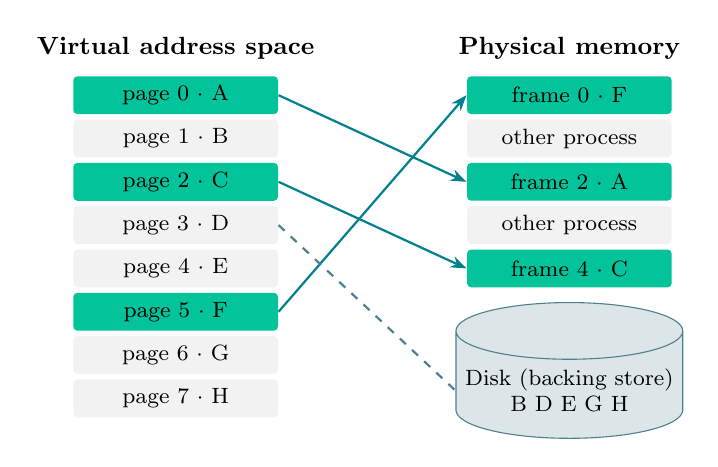
\begin{tikzpicture}[p/.style={rectangle,rounded corners=1.5pt,minimum width=2.6cm,minimum height=0.48cm,font=\footnotesize},
  arr/.style={-{Stealth[length=2mm]},thick,mintdeep}]
\node[font=\small\bfseries] at (0,0.6) {Virtual address space};
\foreach \i/\l in {0/A,1/B,2/C,3/D,4/E,5/F,6/G,7/H} {
  \ifnum\i=0 \def\c{mint}\else\ifnum\i=2 \def\c{mint}\else\ifnum\i=5 \def\c{mint}\else\def\c{light}\fi\fi\fi
  \node[p,fill=\c] (v\i) at (0,-0.55*\i) {page \i\ $\cdot$ \l};
}
\node[font=\small\bfseries] at (5,0.6) {Physical memory};
\foreach \i/\l/\c in {0/{frame 0 $\cdot$ F}/mint,1/{other process}/light,2/{frame 2 $\cdot$ A}/mint,3/{other process}/light,4/{frame 4 $\cdot$ C}/mint}
  \node[p,fill=\c] (f\i) at (5,-0.55*\i) {\l};
\draw[arr] (v0.east) -- (f2.west);
\draw[arr] (v2.east) -- (f4.west);
\draw[arr] (v5.east) -- (f0.west);
\node[cylinder,shape border rotate=90,aspect=0.25,draw=slate,fill=slate!20,minimum width=2.6cm,minimum height=1.5cm,align=center,font=\footnotesize] (d) at (5,-3.75) {Disk (backing store)\\B D E G H};
\draw[dashed,slate,thick] (v3.east) -- (d.west);
\end{tikzpicture}
\caption{Only pages A, C and F are in RAM; the other pages of the program wait on the disk.}
\end{figure}

The benefits are considerable:
\begin{itemize}
  \item A program is no longer limited by the size of physical memory. (On 64-bit Linux, each process has a virtual address space of $128$~TiB.)
  \item Each process occupies less RAM, so more processes fit in memory at once: the \emph{degree of multiprogramming} rises and with it CPU utilisation (Weeks~1 and~4).
  \item Less I/O is needed to load or swap a program, so programs start faster.
  \item Pages can be shared between processes (shared libraries, and copy-on-write after \cmd{fork()}, Section~\ref{sec:cow}).
\end{itemize}

% =====================================================================
\section{Demand Paging}

\subsection{Lazy loading}

How does the OS decide which pages to put in RAM? The simplest strategy is to load the whole program before it starts. The alternative, used by every modern general-purpose OS, is \term{demand paging}: a page is loaded only when it is first referenced. This is an instance of a general programming idea called \emph{lazy loading}: never do work before it is needed.

Compared with loading the whole program eagerly, demand paging needs less I/O and less memory, starts programs faster and lets more processes fit in RAM. The price is that the first use of each page causes a \emph{page fault}.

The part of the OS that moves individual pages between disk and memory is called the \term{pager}. (The older word \emph{swapper} refers to moving \emph{whole processes}.) In \emph{pure} demand paging a process starts with no pages in memory at all; its very first instruction causes a fault.

\subsection{The valid--invalid bit}

The hardware needs a way to tell whether a page is in memory. Each page-table entry has a \term{valid--invalid bit}:
\begin{itemize}
  \item \textbf{v (valid):} the page belongs to the process \emph{and} is in a frame; the entry holds the frame number.
  \item \textbf{i (invalid):} the page is either not in memory at the moment, or not part of the process's address space at all.
\end{itemize}
Initially, every entry is set to i. While a process accesses only valid pages, it runs exactly as in Week~6, at full speed.

\begin{figure}[H]
\centering
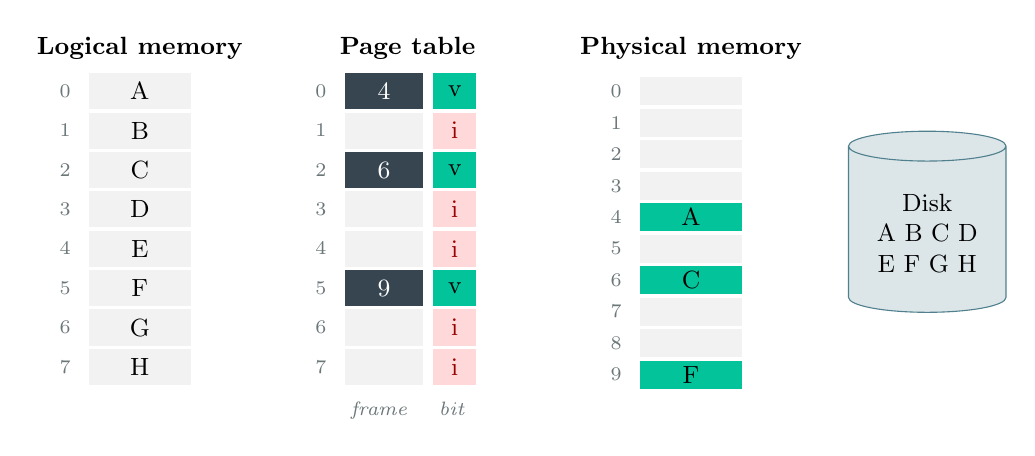
\begin{tikzpicture}[c/.style={rectangle,minimum width=1.3cm,minimum height=0.46cm,font=\small,inner sep=0pt}]
\node[font=\small\bfseries] at (0,0.55) {Logical memory};
\node[font=\small\bfseries] at (3.4,0.55) {Page table};
\node[font=\small\bfseries] at (7.0,0.55) {Physical memory};
\foreach \i/\l in {0/A,1/B,2/C,3/D,4/E,5/F,6/G,7/H} {
  \node[font=\scriptsize,text=muted] at (-0.95,-0.5*\i) {\i};
  \node[c,fill=light] at (0,-0.5*\i) {\l};
}
\foreach \i/\f/\b in {0/4/v,1//i,2/6/v,3//i,4//i,5/9/v,6//i,7//i} {
  \node[font=\scriptsize,text=muted] at (2.3,-0.5*\i) {\i};
  \if v\b
    \node[c,fill=charcoal,text=white,minimum width=1.0cm] at (3.1,-0.5*\i) {\f};
    \node[c,fill=mint,minimum width=0.55cm] at (4.0,-0.5*\i) {v};
  \else
    \node[c,fill=light,minimum width=1.0cm] at (3.1,-0.5*\i) {};
    \node[c,fill=red!15,text=red!60!black,minimum width=0.55cm] at (4.0,-0.5*\i) {i};
  \fi
}
\node[font=\scriptsize\itshape,text=muted] at (3.4,-4.05) {frame \quad bit};
\foreach \i in {0,...,9} {
  \node[font=\scriptsize,text=muted] at (6.05,-0.4*\i) {\i};
  \node[c,fill=light,minimum height=0.36cm] (pm\i) at (7.0,-0.4*\i) {};
}
\node[c,fill=mint,minimum height=0.36cm] at (7.0,-1.6) {A};
\node[c,fill=mint,minimum height=0.36cm] at (7.0,-2.4) {C};
\node[c,fill=mint,minimum height=0.36cm] at (7.0,-3.6) {F};
\node[cylinder,shape border rotate=90,aspect=0.25,draw=slate,fill=slate!20,minimum width=2.0cm,minimum height=2.3cm,align=center,font=\small] at (10.0,-1.8) {Disk\\A B C D\\E F G H};
\end{tikzpicture}
\caption{Pages A, C and F are in frames 4, 6 and 9 (bit v); all other entries are invalid. Every page has a copy on the disk.}
\end{figure}

\subsection{Handling a page fault}

What happens when the process touches a page whose bit is i? The MMU cannot translate the address, so it raises a \term{page fault}: a trap to the operating system (Week~2). The OS then works through the following steps.

\begin{figure}[H]
\centering
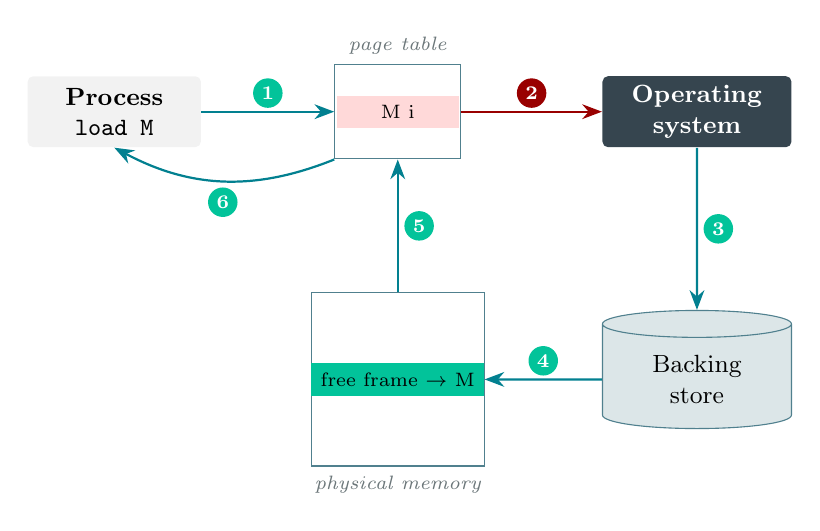
\begin{tikzpicture}[b/.style={rectangle,rounded corners=2pt,minimum height=0.9cm,align=center,font=\small},
  arr/.style={-{Stealth[length=2.5mm]},thick,mintdeep},
  num/.style={circle,fill=mint,text=white,font=\scriptsize\bfseries,inner sep=1.5pt}]
\node[b,fill=light,minimum width=2.2cm] (proc) at (0,0) {\textbf{Process}\\\texttt{load M}};
\node[rectangle,draw=slate,minimum width=1.6cm,minimum height=1.2cm,label={[font=\scriptsize\itshape,text=muted]above:page table}] (pt) at (3.6,0) {};
\node[rectangle,fill=red!15,minimum width=1.55cm,minimum height=0.36cm,font=\scriptsize] at (3.6,0) {M \hfill i};
\node[b,fill=charcoal,text=white,minimum width=2.4cm] (os) at (7.4,0) {\textbf{Operating}\\\textbf{system}};
\node[cylinder,shape border rotate=90,aspect=0.25,draw=slate,fill=slate!20,minimum width=2.4cm,minimum height=1.5cm,align=center,font=\small] (disk) at (7.4,-3.4) {Backing\\store};
\node[rectangle,draw=slate,minimum width=2.2cm,minimum height=2.2cm,label={[font=\scriptsize\itshape,text=muted]below:physical memory}] (pm) at (3.6,-3.4) {};
\node[rectangle,fill=mint,minimum width=2.1cm,minimum height=0.42cm,font=\scriptsize] (ff) at (3.6,-3.4) {free frame $\to$ M};
\draw[arr] (proc.east) -- node[num,above=1pt]{1} (pt.west);
\draw[arr,red!60!black] (pt.east) -- node[num,fill=red!60!black,above=1pt]{2} (os.west);
\draw[arr] (os.south) -- node[num,right=2pt]{3} (disk.north);
\draw[arr] (disk.west) -- node[num,above=1pt]{4} (ff.east);
\draw[arr] (pm.north) -- node[num,right=2pt]{5} (pt.south);
\draw[arr] (pt.south west) to[bend left=25] node[num,below=2pt]{6} (proc.south);
\end{tikzpicture}
\caption{The six steps of page-fault handling.}
\label{fig:pf}
\end{figure}

\begin{enumerate}[leftmargin=1.4em]
  \item \textbf{Reference.} The process executes an instruction that refers to page M. Its page-table entry says i.
  \item \textbf{Trap.} The MMU raises a page fault. The OS saves the process state and checks an internal table: is the address legal at all? If not, the process is terminated (on Linux: \emph{segmentation fault}). If it is legal but not in memory, continue.
  \item \textbf{Locate.} The OS finds where page M is on the backing store and finds a free frame (if there is none, it must \emph{replace} a page, Section~\ref{sec:repl}).
  \item \textbf{Read.} It schedules a disk read of the page into the frame. This takes milliseconds, so meanwhile the CPU scheduler (Week~4) runs another process; the faulting process is in the \emph{waiting} state (Week~3).
  \item \textbf{Update.} When the disk interrupt arrives, the OS writes the frame number into the page-table entry and sets the bit to v.
  \item \textbf{Restart.} The process is made ready again, and the instruction that caused the fault is \emph{restarted from the beginning}. This time the access succeeds; the process cannot tell that anything happened (except that it was slower).
\end{enumerate}

\paragraph{Minor and major faults.} Not every page fault needs the disk. If the page is brand-new memory (for example the first touch of a \cmd{malloc}'ed array), the OS only has to find a free frame and fill it with zeros. Linux calls this a \term{minor fault}. A \term{major fault} needs disk I/O, for example to read a page of a program file or a page that was swapped out. Major faults are thousands of times more expensive.

\subsection{Effective access time with page faults}

Let $p$ be the \term{page-fault rate}, the probability that a memory access causes a page fault ($0 \le p \le 1$). With memory access time $t_m$ and page-fault service time $t_{\text{fault}}$, the \term{effective access time} is the weighted average
\[
\text{EAT} = (1-p)\, t_m + p\, t_{\text{fault}} .
\]
This has exactly the same structure as the TLB formula of Week~6: a fast case weighted by its probability plus a slow case weighted by its probability. The fault service time includes the trap, saving the state, the disk read (by far the largest part) and restarting the process.

\begin{example}[EAT with page faults]
Take $t_m = 200\ \text{ns}$ and $t_{\text{fault}} = 8\ \text{ms} = 8\,000\,000\ \text{ns}$, and suppose one access in a thousand faults, $p = 0.001$:
\begin{align*}
\text{EAT} &= 0.999 \times 200\ \text{ns} + 0.001 \times 8\,000\,000\ \text{ns} \\
           &= 199.8\ \text{ns} + 8\,000\ \text{ns} = 8\,199.8\ \text{ns} \approx 8.2\ \mu\text{s}.
\end{align*}
Memory has become $8199.8/200 \approx 41$ times slower!

\textbf{How small must $p$ be for a slow-down below $10\%$?} We need $\text{EAT} < 1.1\, t_m = 220\ \text{ns}$:
\[
200 + p\,(8\,000\,000 - 200) < 220
\quad\Longrightarrow\quad
p < \frac{20}{7\,999\,800} \approx 2.5 \times 10^{-6}.
\]
That is at most one page fault per $1/p \approx 400\,000$ memory accesses. (Numbers checked with \cmd{code/page\_replacement.py}.)
\end{example}

The lesson: the page-fault rate must be extremely small, and it \emph{is} small in practice only because of locality. With an SSD ($t_{\text{fault}}$ of the order of $0.1$~ms) the penalty is smaller, but the same reasoning applies.

\subsection{Copy-on-write}
\label{sec:cow}

In Week~3 we met \cmd{fork()}, which creates a child process as a copy of its parent. Copying every page of the parent would be slow, and often pointless: many children immediately call \cmd{exec()} and replace their whole memory with a new program. Virtual memory offers a better solution, \term{copy-on-write} (COW).

\begin{figure}[H]
\centering
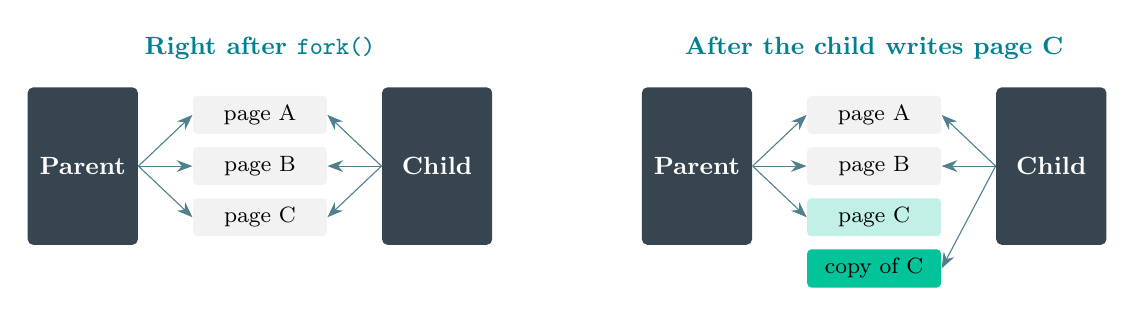
\begin{tikzpicture}[pr/.style={rectangle,rounded corners=2pt,fill=charcoal,text=white,minimum width=1.4cm,minimum height=2.0cm,font=\small\bfseries},
  pg/.style={rectangle,rounded corners=1.5pt,minimum width=1.7cm,minimum height=0.45cm,font=\footnotesize},
  arr/.style={-{Stealth[length=2mm]},slate}]
\begin{scope}
\node[font=\small\bfseries,text=mintdeep] at (2.25,1.5) {Right after \texttt{fork()}};
\node[pr] (p) at (0,0) {Parent}; \node[pr] (c) at (4.5,0) {Child};
\foreach \i/\t in {0/page A,1/page B,2/page C} { \node[pg,fill=light] (a\i) at (2.25,0.65-0.65*\i) {\t};
  \draw[arr] (p.east) -- (a\i.west); \draw[arr] (c.west) -- (a\i.east); }
\end{scope}
\begin{scope}[xshift=7.8cm]
\node[font=\small\bfseries,text=mintdeep] at (2.25,1.5) {After the child writes page C};
\node[pr] (p) at (0,0) {Parent}; \node[pr] (c) at (4.5,0) {Child};
\foreach \i/\t/\f in {0/page A/light,1/page B/light,2/page C/mint!25,3/copy of C/mint} \node[pg,fill=\f] (b\i) at (2.25,0.65-0.65*\i) {\t};
\foreach \i in {0,1,2} \draw[arr] (p.east) -- (b\i.west);
\foreach \i in {0,1,3} \draw[arr] (c.west) -- (b\i.east);
\end{scope}
\end{tikzpicture}
\caption{Copy-on-write: pages are shared until one process writes; only the written page is copied.}
\end{figure}

After \cmd{fork()}, parent and child share all their pages, and the OS marks them read-only. Reading is free. When either process \emph{writes} to a shared page, the hardware raises a protection fault; the OS copies just that page, gives the writer its own copy (now writable) and restarts the write. Pages that are never written are never copied. The mechanism is the same trap-and-restart we used for demand paging.

\subsection{Hands-on: watching page faults happen}

The programs in this section are in the \texttt{code/} folder next to these notes. Compile everything with \cmd{make} (which uses \cmd{gcc -Wall -O2}).

\paragraph{Example 1: demand paging.} The program allocates $64$~MB with \cmd{malloc()}, then writes one byte into every page twice. The kernel counts page faults for each process; \cmd{getrusage()} reads the counter. The listing shows the core of the program; the complete version, which also prints the results, is \cmd{page\_faults.c}.

\lstinputlisting[caption={}]{../code/page_faults_excerpt.c}

Output on our test machine (Linux, $4$~KB pages):
\Needspace{7\baselineskip}
\begin{lstlisting}[style=term]
$ ./page_faults
page size 4096 bytes; array 64 MB = 16384 pages
after malloc       :      1 new faults
first touch (write):  16383 new faults
second touch       :      0 new faults
\end{lstlisting}

Reading the output:
\begin{itemize}
  \item \cmd{malloc()} itself causes only $1$ fault: it reserves \emph{virtual} space and writes only a small bookkeeping header (into the first page).
  \item The first pass faults once for each page it touches: $16\,383$ faults, plus the $1$ page already touched by \cmd{malloc} gives all $16\,384$ pages.
  \item The second pass causes $0$ faults: every page is now resident.
\end{itemize}
These are all \emph{minor} faults: the kernel only had to hand out zero-filled frames. The tool \cmd{/usr/bin/time -v} reports the counters for the whole run (including the faults for loading the program and the C library):
\Needspace{7\baselineskip}
\begin{lstlisting}[style=term]
$ /usr/bin/time -v ./page_faults
...
   Maximum resident set size (kbytes): 66964
   Major (requiring I/O) page faults: 0
   Minor (reclaiming a frame) page faults: 16463
\end{lstlisting}
On systems where \emph{transparent huge pages} are enabled for all memory, the kernel may map $2$~MB pages instead and you will see far fewer faults. (Install the tool with \cmd{sudo apt install time} if \cmd{/usr/bin/time} is missing.)

\paragraph{Example 2: copy-on-write.} The parent fills a $32$~MB buffer and forks. The child first reads every page, then writes every page. The listing shows the core of the program; the complete version, with the same \cmd{minor\_faults()} helper as Example~1, is \cmd{code/cow\_fork.c}.

\lstinputlisting[caption={}]{../code/cow_fork_excerpt.c}

\Needspace{7\baselineskip}
\begin{lstlisting}[style=term]
$ ./cow_fork
buffer: 8192 pages of 4096 bytes
child read  all pages:      0 faults
child write all pages:   8192 faults (copy-on-write)
parent still sees  'A'  (its copy was never changed)
\end{lstlisting}

Reading the shared pages costs nothing; writing costs exactly one fault per page, $8192$ in total, because each page is copied on its first write. The parent still sees its original data. (The \cmd{fflush(stdout)} before \cmd{fork()} matters: without it, text still sitting in the parent's output buffer would be copied into the child and printed twice.)

% =====================================================================
\section{Page Replacement}
\label{sec:repl}

\subsection{When memory is full}

The OS deliberately \emph{over-allocates} memory: the virtual memory of all processes together is larger than RAM, on the bet that not all pages are needed at once. Sooner or later a page fault occurs and there is no free frame. The OS must then choose a \term{victim} page to remove. The page-fault routine becomes:

\begin{enumerate}[leftmargin=1.4em]
  \item Find the location of the wanted page on the disk.
  \item Find a free frame. If there is none, use a \term{page-replacement algorithm} to select a victim frame; if the victim has been modified, write it to the disk; mark its page-table entry invalid.
  \item Read the wanted page into the freed frame; update the page table.
  \item Restart the process.
\end{enumerate}

\paragraph{The modify (dirty) bit.} Without care, a replacement costs \emph{two} disk transfers: one to write the victim out and one to read the new page in. The hardware therefore keeps a \term{modify bit} (dirty bit) for every page, set automatically whenever the page is written. A \emph{clean} victim, such as a page of program code, already has an identical copy on the disk and can simply be dropped.

\paragraph{How we compare algorithms.} We run each algorithm on the same \term{reference string}, the sequence of page numbers that a program references, with the same number of frames, and count page faults. Throughout this section we use the classic string
\[
7,\,0,\,1,\,2,\,0,\,3,\,0,\,4,\,2,\,3,\,0,\,3,\,2,\,1,\,2,\,0,\,1,\,7,\,0,\,1
\]
with $3$ frames, all initially empty. In the tables below, mint marks the page just loaded, pale columns are page faults, and grey columns are hits. All tables were produced by the Python simulator in the \texttt{code/} folder (\cmd{page\_replacement.py}).

\subsection{FIFO: first in, first out}

The victim is the page that has been in memory the longest. FIFO is trivial to implement with a queue of page numbers.

\begin{figure}[H]
\centering
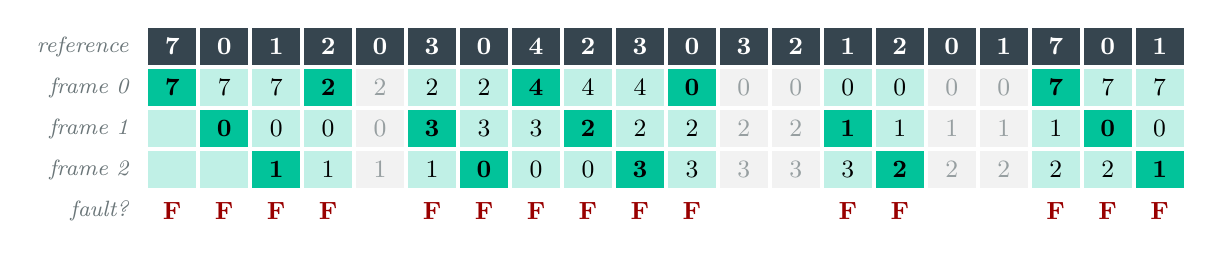
\begin{tikzpicture}[c/.style={rectangle,minimum width=0.61cm,minimum height=0.47cm,inner sep=0pt,font=\small}]
\node[anchor=east,font=\footnotesize\itshape,text=muted] at (-0.1,0.00) {reference};
\node[anchor=east,font=\footnotesize\itshape,text=muted] at (-0.1,-0.52) {frame 0};
\node[anchor=east,font=\footnotesize\itshape,text=muted] at (-0.1,-1.04) {frame 1};
\node[anchor=east,font=\footnotesize\itshape,text=muted] at (-0.1,-1.56) {frame 2};
\node[anchor=east,font=\footnotesize\itshape,text=muted] at (-0.1,-2.08) {fault?};
\node[c,fill=charcoal,text=white,font=\small\bfseries] at (0.33,0) {7};
\node[c,fill=mint,text=black] at (0.33,-0.52) {\bfseries7};
\node[c,fill=mint!25,text=black] at (0.33,-1.04) {};
\node[c,fill=mint!25,text=black] at (0.33,-1.56) {};
\node[c,text=red!60!black,font=\small\bfseries] at (0.33,-2.08) {F};
\node[c,fill=charcoal,text=white,font=\small\bfseries] at (0.99,0) {0};
\node[c,fill=mint!25,text=black] at (0.99,-0.52) {7};
\node[c,fill=mint,text=black] at (0.99,-1.04) {\bfseries0};
\node[c,fill=mint!25,text=black] at (0.99,-1.56) {};
\node[c,text=red!60!black,font=\small\bfseries] at (0.99,-2.08) {F};
\node[c,fill=charcoal,text=white,font=\small\bfseries] at (1.65,0) {1};
\node[c,fill=mint!25,text=black] at (1.65,-0.52) {7};
\node[c,fill=mint!25,text=black] at (1.65,-1.04) {0};
\node[c,fill=mint,text=black] at (1.65,-1.56) {\bfseries1};
\node[c,text=red!60!black,font=\small\bfseries] at (1.65,-2.08) {F};
\node[c,fill=charcoal,text=white,font=\small\bfseries] at (2.31,0) {2};
\node[c,fill=mint,text=black] at (2.31,-0.52) {\bfseries2};
\node[c,fill=mint!25,text=black] at (2.31,-1.04) {0};
\node[c,fill=mint!25,text=black] at (2.31,-1.56) {1};
\node[c,text=red!60!black,font=\small\bfseries] at (2.31,-2.08) {F};
\node[c,fill=charcoal,text=white,font=\small\bfseries] at (2.97,0) {0};
\node[c,fill=light,text=muted!70] at (2.97,-0.52) {2};
\node[c,fill=light,text=muted!70] at (2.97,-1.04) {0};
\node[c,fill=light,text=muted!70] at (2.97,-1.56) {1};
\node[c,fill=charcoal,text=white,font=\small\bfseries] at (3.63,0) {3};
\node[c,fill=mint!25,text=black] at (3.63,-0.52) {2};
\node[c,fill=mint,text=black] at (3.63,-1.04) {\bfseries3};
\node[c,fill=mint!25,text=black] at (3.63,-1.56) {1};
\node[c,text=red!60!black,font=\small\bfseries] at (3.63,-2.08) {F};
\node[c,fill=charcoal,text=white,font=\small\bfseries] at (4.29,0) {0};
\node[c,fill=mint!25,text=black] at (4.29,-0.52) {2};
\node[c,fill=mint!25,text=black] at (4.29,-1.04) {3};
\node[c,fill=mint,text=black] at (4.29,-1.56) {\bfseries0};
\node[c,text=red!60!black,font=\small\bfseries] at (4.29,-2.08) {F};
\node[c,fill=charcoal,text=white,font=\small\bfseries] at (4.95,0) {4};
\node[c,fill=mint,text=black] at (4.95,-0.52) {\bfseries4};
\node[c,fill=mint!25,text=black] at (4.95,-1.04) {3};
\node[c,fill=mint!25,text=black] at (4.95,-1.56) {0};
\node[c,text=red!60!black,font=\small\bfseries] at (4.95,-2.08) {F};
\node[c,fill=charcoal,text=white,font=\small\bfseries] at (5.61,0) {2};
\node[c,fill=mint!25,text=black] at (5.61,-0.52) {4};
\node[c,fill=mint,text=black] at (5.61,-1.04) {\bfseries2};
\node[c,fill=mint!25,text=black] at (5.61,-1.56) {0};
\node[c,text=red!60!black,font=\small\bfseries] at (5.61,-2.08) {F};
\node[c,fill=charcoal,text=white,font=\small\bfseries] at (6.27,0) {3};
\node[c,fill=mint!25,text=black] at (6.27,-0.52) {4};
\node[c,fill=mint!25,text=black] at (6.27,-1.04) {2};
\node[c,fill=mint,text=black] at (6.27,-1.56) {\bfseries3};
\node[c,text=red!60!black,font=\small\bfseries] at (6.27,-2.08) {F};
\node[c,fill=charcoal,text=white,font=\small\bfseries] at (6.93,0) {0};
\node[c,fill=mint,text=black] at (6.93,-0.52) {\bfseries0};
\node[c,fill=mint!25,text=black] at (6.93,-1.04) {2};
\node[c,fill=mint!25,text=black] at (6.93,-1.56) {3};
\node[c,text=red!60!black,font=\small\bfseries] at (6.93,-2.08) {F};
\node[c,fill=charcoal,text=white,font=\small\bfseries] at (7.59,0) {3};
\node[c,fill=light,text=muted!70] at (7.59,-0.52) {0};
\node[c,fill=light,text=muted!70] at (7.59,-1.04) {2};
\node[c,fill=light,text=muted!70] at (7.59,-1.56) {3};
\node[c,fill=charcoal,text=white,font=\small\bfseries] at (8.25,0) {2};
\node[c,fill=light,text=muted!70] at (8.25,-0.52) {0};
\node[c,fill=light,text=muted!70] at (8.25,-1.04) {2};
\node[c,fill=light,text=muted!70] at (8.25,-1.56) {3};
\node[c,fill=charcoal,text=white,font=\small\bfseries] at (8.91,0) {1};
\node[c,fill=mint!25,text=black] at (8.91,-0.52) {0};
\node[c,fill=mint,text=black] at (8.91,-1.04) {\bfseries1};
\node[c,fill=mint!25,text=black] at (8.91,-1.56) {3};
\node[c,text=red!60!black,font=\small\bfseries] at (8.91,-2.08) {F};
\node[c,fill=charcoal,text=white,font=\small\bfseries] at (9.57,0) {2};
\node[c,fill=mint!25,text=black] at (9.57,-0.52) {0};
\node[c,fill=mint!25,text=black] at (9.57,-1.04) {1};
\node[c,fill=mint,text=black] at (9.57,-1.56) {\bfseries2};
\node[c,text=red!60!black,font=\small\bfseries] at (9.57,-2.08) {F};
\node[c,fill=charcoal,text=white,font=\small\bfseries] at (10.23,0) {0};
\node[c,fill=light,text=muted!70] at (10.23,-0.52) {0};
\node[c,fill=light,text=muted!70] at (10.23,-1.04) {1};
\node[c,fill=light,text=muted!70] at (10.23,-1.56) {2};
\node[c,fill=charcoal,text=white,font=\small\bfseries] at (10.89,0) {1};
\node[c,fill=light,text=muted!70] at (10.89,-0.52) {0};
\node[c,fill=light,text=muted!70] at (10.89,-1.04) {1};
\node[c,fill=light,text=muted!70] at (10.89,-1.56) {2};
\node[c,fill=charcoal,text=white,font=\small\bfseries] at (11.55,0) {7};
\node[c,fill=mint,text=black] at (11.55,-0.52) {\bfseries7};
\node[c,fill=mint!25,text=black] at (11.55,-1.04) {1};
\node[c,fill=mint!25,text=black] at (11.55,-1.56) {2};
\node[c,text=red!60!black,font=\small\bfseries] at (11.55,-2.08) {F};
\node[c,fill=charcoal,text=white,font=\small\bfseries] at (12.21,0) {0};
\node[c,fill=mint!25,text=black] at (12.21,-0.52) {7};
\node[c,fill=mint,text=black] at (12.21,-1.04) {\bfseries0};
\node[c,fill=mint!25,text=black] at (12.21,-1.56) {2};
\node[c,text=red!60!black,font=\small\bfseries] at (12.21,-2.08) {F};
\node[c,fill=charcoal,text=white,font=\small\bfseries] at (12.87,0) {1};
\node[c,fill=mint!25,text=black] at (12.87,-0.52) {7};
\node[c,fill=mint!25,text=black] at (12.87,-1.04) {0};
\node[c,fill=mint,text=black] at (12.87,-1.56) {\bfseries1};
\node[c,text=red!60!black,font=\small\bfseries] at (12.87,-2.08) {F};
\end{tikzpicture}
\caption{FIFO with 3 frames: \textbf{15 page faults}.}
\end{figure}

The first three faults are \term{compulsory} (cold-start) faults: no algorithm can avoid loading 7, 0 and 1 the first time. Then 2 replaces 7 (the oldest), 0 is a hit, and 3 replaces 0, because 0 is now the oldest page --- even though 0 is needed again at the very next reference. FIFO knows when a page arrived, not whether it is still being used.

\subsection{OPT: the optimal algorithm}

The victim is the page that \emph{will not be used for the longest time} in the future. This algorithm (OPT or MIN, Bélády 1966) gives the lowest possible number of page faults for any reference string and number of frames.

\begin{figure}[H]
\centering
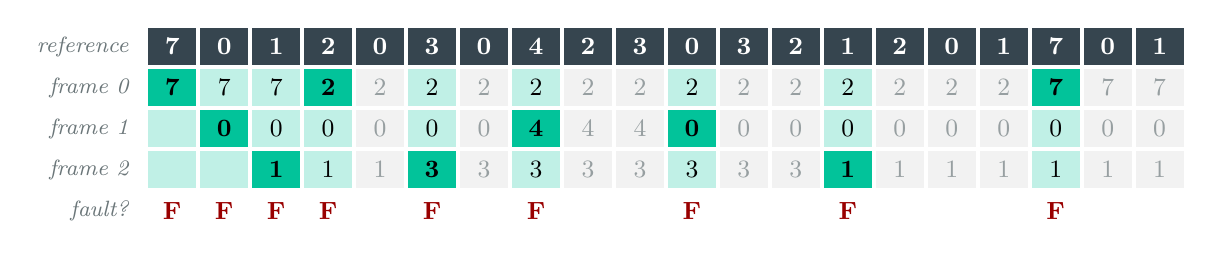
\begin{tikzpicture}[c/.style={rectangle,minimum width=0.61cm,minimum height=0.47cm,inner sep=0pt,font=\small}]
\node[anchor=east,font=\footnotesize\itshape,text=muted] at (-0.1,0.00) {reference};
\node[anchor=east,font=\footnotesize\itshape,text=muted] at (-0.1,-0.52) {frame 0};
\node[anchor=east,font=\footnotesize\itshape,text=muted] at (-0.1,-1.04) {frame 1};
\node[anchor=east,font=\footnotesize\itshape,text=muted] at (-0.1,-1.56) {frame 2};
\node[anchor=east,font=\footnotesize\itshape,text=muted] at (-0.1,-2.08) {fault?};
\node[c,fill=charcoal,text=white,font=\small\bfseries] at (0.33,0) {7};
\node[c,fill=mint,text=black] at (0.33,-0.52) {\bfseries7};
\node[c,fill=mint!25,text=black] at (0.33,-1.04) {};
\node[c,fill=mint!25,text=black] at (0.33,-1.56) {};
\node[c,text=red!60!black,font=\small\bfseries] at (0.33,-2.08) {F};
\node[c,fill=charcoal,text=white,font=\small\bfseries] at (0.99,0) {0};
\node[c,fill=mint!25,text=black] at (0.99,-0.52) {7};
\node[c,fill=mint,text=black] at (0.99,-1.04) {\bfseries0};
\node[c,fill=mint!25,text=black] at (0.99,-1.56) {};
\node[c,text=red!60!black,font=\small\bfseries] at (0.99,-2.08) {F};
\node[c,fill=charcoal,text=white,font=\small\bfseries] at (1.65,0) {1};
\node[c,fill=mint!25,text=black] at (1.65,-0.52) {7};
\node[c,fill=mint!25,text=black] at (1.65,-1.04) {0};
\node[c,fill=mint,text=black] at (1.65,-1.56) {\bfseries1};
\node[c,text=red!60!black,font=\small\bfseries] at (1.65,-2.08) {F};
\node[c,fill=charcoal,text=white,font=\small\bfseries] at (2.31,0) {2};
\node[c,fill=mint,text=black] at (2.31,-0.52) {\bfseries2};
\node[c,fill=mint!25,text=black] at (2.31,-1.04) {0};
\node[c,fill=mint!25,text=black] at (2.31,-1.56) {1};
\node[c,text=red!60!black,font=\small\bfseries] at (2.31,-2.08) {F};
\node[c,fill=charcoal,text=white,font=\small\bfseries] at (2.97,0) {0};
\node[c,fill=light,text=muted!70] at (2.97,-0.52) {2};
\node[c,fill=light,text=muted!70] at (2.97,-1.04) {0};
\node[c,fill=light,text=muted!70] at (2.97,-1.56) {1};
\node[c,fill=charcoal,text=white,font=\small\bfseries] at (3.63,0) {3};
\node[c,fill=mint!25,text=black] at (3.63,-0.52) {2};
\node[c,fill=mint!25,text=black] at (3.63,-1.04) {0};
\node[c,fill=mint,text=black] at (3.63,-1.56) {\bfseries3};
\node[c,text=red!60!black,font=\small\bfseries] at (3.63,-2.08) {F};
\node[c,fill=charcoal,text=white,font=\small\bfseries] at (4.29,0) {0};
\node[c,fill=light,text=muted!70] at (4.29,-0.52) {2};
\node[c,fill=light,text=muted!70] at (4.29,-1.04) {0};
\node[c,fill=light,text=muted!70] at (4.29,-1.56) {3};
\node[c,fill=charcoal,text=white,font=\small\bfseries] at (4.95,0) {4};
\node[c,fill=mint!25,text=black] at (4.95,-0.52) {2};
\node[c,fill=mint,text=black] at (4.95,-1.04) {\bfseries4};
\node[c,fill=mint!25,text=black] at (4.95,-1.56) {3};
\node[c,text=red!60!black,font=\small\bfseries] at (4.95,-2.08) {F};
\node[c,fill=charcoal,text=white,font=\small\bfseries] at (5.61,0) {2};
\node[c,fill=light,text=muted!70] at (5.61,-0.52) {2};
\node[c,fill=light,text=muted!70] at (5.61,-1.04) {4};
\node[c,fill=light,text=muted!70] at (5.61,-1.56) {3};
\node[c,fill=charcoal,text=white,font=\small\bfseries] at (6.27,0) {3};
\node[c,fill=light,text=muted!70] at (6.27,-0.52) {2};
\node[c,fill=light,text=muted!70] at (6.27,-1.04) {4};
\node[c,fill=light,text=muted!70] at (6.27,-1.56) {3};
\node[c,fill=charcoal,text=white,font=\small\bfseries] at (6.93,0) {0};
\node[c,fill=mint!25,text=black] at (6.93,-0.52) {2};
\node[c,fill=mint,text=black] at (6.93,-1.04) {\bfseries0};
\node[c,fill=mint!25,text=black] at (6.93,-1.56) {3};
\node[c,text=red!60!black,font=\small\bfseries] at (6.93,-2.08) {F};
\node[c,fill=charcoal,text=white,font=\small\bfseries] at (7.59,0) {3};
\node[c,fill=light,text=muted!70] at (7.59,-0.52) {2};
\node[c,fill=light,text=muted!70] at (7.59,-1.04) {0};
\node[c,fill=light,text=muted!70] at (7.59,-1.56) {3};
\node[c,fill=charcoal,text=white,font=\small\bfseries] at (8.25,0) {2};
\node[c,fill=light,text=muted!70] at (8.25,-0.52) {2};
\node[c,fill=light,text=muted!70] at (8.25,-1.04) {0};
\node[c,fill=light,text=muted!70] at (8.25,-1.56) {3};
\node[c,fill=charcoal,text=white,font=\small\bfseries] at (8.91,0) {1};
\node[c,fill=mint!25,text=black] at (8.91,-0.52) {2};
\node[c,fill=mint!25,text=black] at (8.91,-1.04) {0};
\node[c,fill=mint,text=black] at (8.91,-1.56) {\bfseries1};
\node[c,text=red!60!black,font=\small\bfseries] at (8.91,-2.08) {F};
\node[c,fill=charcoal,text=white,font=\small\bfseries] at (9.57,0) {2};
\node[c,fill=light,text=muted!70] at (9.57,-0.52) {2};
\node[c,fill=light,text=muted!70] at (9.57,-1.04) {0};
\node[c,fill=light,text=muted!70] at (9.57,-1.56) {1};
\node[c,fill=charcoal,text=white,font=\small\bfseries] at (10.23,0) {0};
\node[c,fill=light,text=muted!70] at (10.23,-0.52) {2};
\node[c,fill=light,text=muted!70] at (10.23,-1.04) {0};
\node[c,fill=light,text=muted!70] at (10.23,-1.56) {1};
\node[c,fill=charcoal,text=white,font=\small\bfseries] at (10.89,0) {1};
\node[c,fill=light,text=muted!70] at (10.89,-0.52) {2};
\node[c,fill=light,text=muted!70] at (10.89,-1.04) {0};
\node[c,fill=light,text=muted!70] at (10.89,-1.56) {1};
\node[c,fill=charcoal,text=white,font=\small\bfseries] at (11.55,0) {7};
\node[c,fill=mint,text=black] at (11.55,-0.52) {\bfseries7};
\node[c,fill=mint!25,text=black] at (11.55,-1.04) {0};
\node[c,fill=mint!25,text=black] at (11.55,-1.56) {1};
\node[c,text=red!60!black,font=\small\bfseries] at (11.55,-2.08) {F};
\node[c,fill=charcoal,text=white,font=\small\bfseries] at (12.21,0) {0};
\node[c,fill=light,text=muted!70] at (12.21,-0.52) {7};
\node[c,fill=light,text=muted!70] at (12.21,-1.04) {0};
\node[c,fill=light,text=muted!70] at (12.21,-1.56) {1};
\node[c,fill=charcoal,text=white,font=\small\bfseries] at (12.87,0) {1};
\node[c,fill=light,text=muted!70] at (12.87,-0.52) {7};
\node[c,fill=light,text=muted!70] at (12.87,-1.04) {0};
\node[c,fill=light,text=muted!70] at (12.87,-1.56) {1};
\end{tikzpicture}
\caption{OPT with 3 frames: \textbf{9 page faults}, the minimum.}
\end{figure}

For example, at the reference to page 4 (position 8), the frames hold 2, 0 and 3. Looking ahead, 2 is used next at position 9, 3 at position 10 and 0 at position 11, so 0 is replaced. The catch is obvious: the OS cannot know the future reference string. OPT is used as a \emph{yardstick}: ``our algorithm is within $10\%$ of optimal on this workload''.

\subsection{LRU: least recently used}

LRU uses the recent past as an estimate of the near future: the victim is the page that has \emph{not been used for the longest time}. Equivalently, it is OPT looking backwards in time.

\begin{figure}[H]
\centering
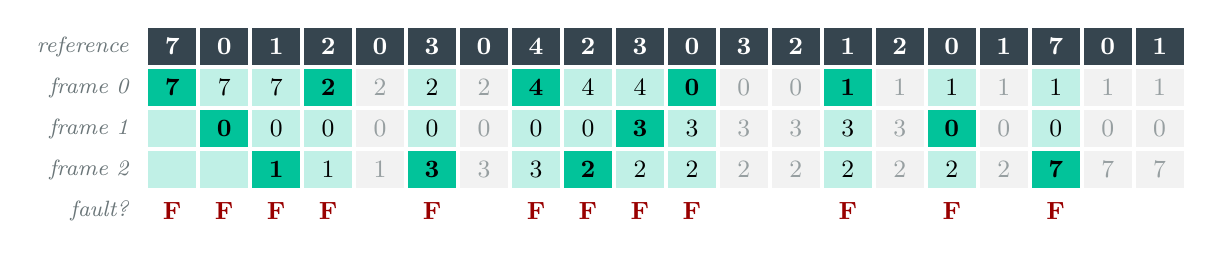
\begin{tikzpicture}[c/.style={rectangle,minimum width=0.61cm,minimum height=0.47cm,inner sep=0pt,font=\small}]
\node[anchor=east,font=\footnotesize\itshape,text=muted] at (-0.1,0.00) {reference};
\node[anchor=east,font=\footnotesize\itshape,text=muted] at (-0.1,-0.52) {frame 0};
\node[anchor=east,font=\footnotesize\itshape,text=muted] at (-0.1,-1.04) {frame 1};
\node[anchor=east,font=\footnotesize\itshape,text=muted] at (-0.1,-1.56) {frame 2};
\node[anchor=east,font=\footnotesize\itshape,text=muted] at (-0.1,-2.08) {fault?};
\node[c,fill=charcoal,text=white,font=\small\bfseries] at (0.33,0) {7};
\node[c,fill=mint,text=black] at (0.33,-0.52) {\bfseries7};
\node[c,fill=mint!25,text=black] at (0.33,-1.04) {};
\node[c,fill=mint!25,text=black] at (0.33,-1.56) {};
\node[c,text=red!60!black,font=\small\bfseries] at (0.33,-2.08) {F};
\node[c,fill=charcoal,text=white,font=\small\bfseries] at (0.99,0) {0};
\node[c,fill=mint!25,text=black] at (0.99,-0.52) {7};
\node[c,fill=mint,text=black] at (0.99,-1.04) {\bfseries0};
\node[c,fill=mint!25,text=black] at (0.99,-1.56) {};
\node[c,text=red!60!black,font=\small\bfseries] at (0.99,-2.08) {F};
\node[c,fill=charcoal,text=white,font=\small\bfseries] at (1.65,0) {1};
\node[c,fill=mint!25,text=black] at (1.65,-0.52) {7};
\node[c,fill=mint!25,text=black] at (1.65,-1.04) {0};
\node[c,fill=mint,text=black] at (1.65,-1.56) {\bfseries1};
\node[c,text=red!60!black,font=\small\bfseries] at (1.65,-2.08) {F};
\node[c,fill=charcoal,text=white,font=\small\bfseries] at (2.31,0) {2};
\node[c,fill=mint,text=black] at (2.31,-0.52) {\bfseries2};
\node[c,fill=mint!25,text=black] at (2.31,-1.04) {0};
\node[c,fill=mint!25,text=black] at (2.31,-1.56) {1};
\node[c,text=red!60!black,font=\small\bfseries] at (2.31,-2.08) {F};
\node[c,fill=charcoal,text=white,font=\small\bfseries] at (2.97,0) {0};
\node[c,fill=light,text=muted!70] at (2.97,-0.52) {2};
\node[c,fill=light,text=muted!70] at (2.97,-1.04) {0};
\node[c,fill=light,text=muted!70] at (2.97,-1.56) {1};
\node[c,fill=charcoal,text=white,font=\small\bfseries] at (3.63,0) {3};
\node[c,fill=mint!25,text=black] at (3.63,-0.52) {2};
\node[c,fill=mint!25,text=black] at (3.63,-1.04) {0};
\node[c,fill=mint,text=black] at (3.63,-1.56) {\bfseries3};
\node[c,text=red!60!black,font=\small\bfseries] at (3.63,-2.08) {F};
\node[c,fill=charcoal,text=white,font=\small\bfseries] at (4.29,0) {0};
\node[c,fill=light,text=muted!70] at (4.29,-0.52) {2};
\node[c,fill=light,text=muted!70] at (4.29,-1.04) {0};
\node[c,fill=light,text=muted!70] at (4.29,-1.56) {3};
\node[c,fill=charcoal,text=white,font=\small\bfseries] at (4.95,0) {4};
\node[c,fill=mint,text=black] at (4.95,-0.52) {\bfseries4};
\node[c,fill=mint!25,text=black] at (4.95,-1.04) {0};
\node[c,fill=mint!25,text=black] at (4.95,-1.56) {3};
\node[c,text=red!60!black,font=\small\bfseries] at (4.95,-2.08) {F};
\node[c,fill=charcoal,text=white,font=\small\bfseries] at (5.61,0) {2};
\node[c,fill=mint!25,text=black] at (5.61,-0.52) {4};
\node[c,fill=mint!25,text=black] at (5.61,-1.04) {0};
\node[c,fill=mint,text=black] at (5.61,-1.56) {\bfseries2};
\node[c,text=red!60!black,font=\small\bfseries] at (5.61,-2.08) {F};
\node[c,fill=charcoal,text=white,font=\small\bfseries] at (6.27,0) {3};
\node[c,fill=mint!25,text=black] at (6.27,-0.52) {4};
\node[c,fill=mint,text=black] at (6.27,-1.04) {\bfseries3};
\node[c,fill=mint!25,text=black] at (6.27,-1.56) {2};
\node[c,text=red!60!black,font=\small\bfseries] at (6.27,-2.08) {F};
\node[c,fill=charcoal,text=white,font=\small\bfseries] at (6.93,0) {0};
\node[c,fill=mint,text=black] at (6.93,-0.52) {\bfseries0};
\node[c,fill=mint!25,text=black] at (6.93,-1.04) {3};
\node[c,fill=mint!25,text=black] at (6.93,-1.56) {2};
\node[c,text=red!60!black,font=\small\bfseries] at (6.93,-2.08) {F};
\node[c,fill=charcoal,text=white,font=\small\bfseries] at (7.59,0) {3};
\node[c,fill=light,text=muted!70] at (7.59,-0.52) {0};
\node[c,fill=light,text=muted!70] at (7.59,-1.04) {3};
\node[c,fill=light,text=muted!70] at (7.59,-1.56) {2};
\node[c,fill=charcoal,text=white,font=\small\bfseries] at (8.25,0) {2};
\node[c,fill=light,text=muted!70] at (8.25,-0.52) {0};
\node[c,fill=light,text=muted!70] at (8.25,-1.04) {3};
\node[c,fill=light,text=muted!70] at (8.25,-1.56) {2};
\node[c,fill=charcoal,text=white,font=\small\bfseries] at (8.91,0) {1};
\node[c,fill=mint,text=black] at (8.91,-0.52) {\bfseries1};
\node[c,fill=mint!25,text=black] at (8.91,-1.04) {3};
\node[c,fill=mint!25,text=black] at (8.91,-1.56) {2};
\node[c,text=red!60!black,font=\small\bfseries] at (8.91,-2.08) {F};
\node[c,fill=charcoal,text=white,font=\small\bfseries] at (9.57,0) {2};
\node[c,fill=light,text=muted!70] at (9.57,-0.52) {1};
\node[c,fill=light,text=muted!70] at (9.57,-1.04) {3};
\node[c,fill=light,text=muted!70] at (9.57,-1.56) {2};
\node[c,fill=charcoal,text=white,font=\small\bfseries] at (10.23,0) {0};
\node[c,fill=mint!25,text=black] at (10.23,-0.52) {1};
\node[c,fill=mint,text=black] at (10.23,-1.04) {\bfseries0};
\node[c,fill=mint!25,text=black] at (10.23,-1.56) {2};
\node[c,text=red!60!black,font=\small\bfseries] at (10.23,-2.08) {F};
\node[c,fill=charcoal,text=white,font=\small\bfseries] at (10.89,0) {1};
\node[c,fill=light,text=muted!70] at (10.89,-0.52) {1};
\node[c,fill=light,text=muted!70] at (10.89,-1.04) {0};
\node[c,fill=light,text=muted!70] at (10.89,-1.56) {2};
\node[c,fill=charcoal,text=white,font=\small\bfseries] at (11.55,0) {7};
\node[c,fill=mint!25,text=black] at (11.55,-0.52) {1};
\node[c,fill=mint!25,text=black] at (11.55,-1.04) {0};
\node[c,fill=mint,text=black] at (11.55,-1.56) {\bfseries7};
\node[c,text=red!60!black,font=\small\bfseries] at (11.55,-2.08) {F};
\node[c,fill=charcoal,text=white,font=\small\bfseries] at (12.21,0) {0};
\node[c,fill=light,text=muted!70] at (12.21,-0.52) {1};
\node[c,fill=light,text=muted!70] at (12.21,-1.04) {0};
\node[c,fill=light,text=muted!70] at (12.21,-1.56) {7};
\node[c,fill=charcoal,text=white,font=\small\bfseries] at (12.87,0) {1};
\node[c,fill=light,text=muted!70] at (12.87,-0.52) {1};
\node[c,fill=light,text=muted!70] at (12.87,-1.04) {0};
\node[c,fill=light,text=muted!70] at (12.87,-1.56) {7};
\end{tikzpicture}
\caption{LRU with 3 frames: \textbf{12 page faults}.}
\end{figure}

At the reference to page 4, the frames again hold 2, 0 and 3, but now we look back: 2 was used longest ago, so 2 is replaced (OPT replaced 0). LRU works well because of locality.

Exact LRU needs hardware support on \emph{every} memory access: either a time stamp written into the page-table entry, or a stack of page numbers in which the referenced page is moved to the top. Both are too expensive for real hardware, so systems \emph{approximate} LRU (Section~\ref{sec:clock}).

\subsection{Comparison}

\begin{center}
\renewcommand{\arraystretch}{1.3}
\begin{tabular}{@{}lllll@{}}
\toprule
\textbf{Algorithm} & \textbf{Victim is the page\dots} & \textbf{Faults (3 frames)} & \textbf{Implementable?} & \textbf{Belady's anomaly?} \\
\midrule
FIFO & loaded longest ago & 15 & yes, very cheap & possible \\
OPT & used farthest in the future & 9 & no (needs the future) & never \\
LRU & used longest ago & 12 & approximately & never \\
\bottomrule
\end{tabular}
\end{center}

\textbf{Exam tip:} work column by column and write the frame contents after every reference. For OPT look \emph{forward} in the string, for LRU look \emph{backward}, for FIFO remember only the order of arrival.

\subsection{Belady's anomaly}

Intuition says that giving a process more frames can never increase its number of page faults. For FIFO, intuition is wrong. Consider the reference string $1, 2, 3, 4, 1, 2, 5, 1, 2, 3, 4, 5$:

\begin{figure}[H]
\centering
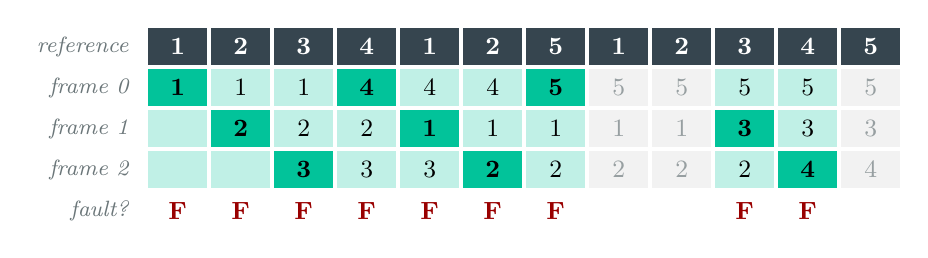
\begin{tikzpicture}[c/.style={rectangle,minimum width=0.75cm,minimum height=0.47cm,inner sep=0pt,font=\small}]
\node[anchor=east,font=\footnotesize\itshape,text=muted] at (-0.1,0.00) {reference};
\node[anchor=east,font=\footnotesize\itshape,text=muted] at (-0.1,-0.52) {frame 0};
\node[anchor=east,font=\footnotesize\itshape,text=muted] at (-0.1,-1.04) {frame 1};
\node[anchor=east,font=\footnotesize\itshape,text=muted] at (-0.1,-1.56) {frame 2};
\node[anchor=east,font=\footnotesize\itshape,text=muted] at (-0.1,-2.08) {fault?};
\node[c,fill=charcoal,text=white,font=\small\bfseries] at (0.40,0) {1};
\node[c,fill=mint,text=black] at (0.40,-0.52) {\bfseries1};
\node[c,fill=mint!25,text=black] at (0.40,-1.04) {};
\node[c,fill=mint!25,text=black] at (0.40,-1.56) {};
\node[c,text=red!60!black,font=\small\bfseries] at (0.40,-2.08) {F};
\node[c,fill=charcoal,text=white,font=\small\bfseries] at (1.20,0) {2};
\node[c,fill=mint!25,text=black] at (1.20,-0.52) {1};
\node[c,fill=mint,text=black] at (1.20,-1.04) {\bfseries2};
\node[c,fill=mint!25,text=black] at (1.20,-1.56) {};
\node[c,text=red!60!black,font=\small\bfseries] at (1.20,-2.08) {F};
\node[c,fill=charcoal,text=white,font=\small\bfseries] at (2.00,0) {3};
\node[c,fill=mint!25,text=black] at (2.00,-0.52) {1};
\node[c,fill=mint!25,text=black] at (2.00,-1.04) {2};
\node[c,fill=mint,text=black] at (2.00,-1.56) {\bfseries3};
\node[c,text=red!60!black,font=\small\bfseries] at (2.00,-2.08) {F};
\node[c,fill=charcoal,text=white,font=\small\bfseries] at (2.80,0) {4};
\node[c,fill=mint,text=black] at (2.80,-0.52) {\bfseries4};
\node[c,fill=mint!25,text=black] at (2.80,-1.04) {2};
\node[c,fill=mint!25,text=black] at (2.80,-1.56) {3};
\node[c,text=red!60!black,font=\small\bfseries] at (2.80,-2.08) {F};
\node[c,fill=charcoal,text=white,font=\small\bfseries] at (3.60,0) {1};
\node[c,fill=mint!25,text=black] at (3.60,-0.52) {4};
\node[c,fill=mint,text=black] at (3.60,-1.04) {\bfseries1};
\node[c,fill=mint!25,text=black] at (3.60,-1.56) {3};
\node[c,text=red!60!black,font=\small\bfseries] at (3.60,-2.08) {F};
\node[c,fill=charcoal,text=white,font=\small\bfseries] at (4.40,0) {2};
\node[c,fill=mint!25,text=black] at (4.40,-0.52) {4};
\node[c,fill=mint!25,text=black] at (4.40,-1.04) {1};
\node[c,fill=mint,text=black] at (4.40,-1.56) {\bfseries2};
\node[c,text=red!60!black,font=\small\bfseries] at (4.40,-2.08) {F};
\node[c,fill=charcoal,text=white,font=\small\bfseries] at (5.20,0) {5};
\node[c,fill=mint,text=black] at (5.20,-0.52) {\bfseries5};
\node[c,fill=mint!25,text=black] at (5.20,-1.04) {1};
\node[c,fill=mint!25,text=black] at (5.20,-1.56) {2};
\node[c,text=red!60!black,font=\small\bfseries] at (5.20,-2.08) {F};
\node[c,fill=charcoal,text=white,font=\small\bfseries] at (6.00,0) {1};
\node[c,fill=light,text=muted!70] at (6.00,-0.52) {5};
\node[c,fill=light,text=muted!70] at (6.00,-1.04) {1};
\node[c,fill=light,text=muted!70] at (6.00,-1.56) {2};
\node[c,fill=charcoal,text=white,font=\small\bfseries] at (6.80,0) {2};
\node[c,fill=light,text=muted!70] at (6.80,-0.52) {5};
\node[c,fill=light,text=muted!70] at (6.80,-1.04) {1};
\node[c,fill=light,text=muted!70] at (6.80,-1.56) {2};
\node[c,fill=charcoal,text=white,font=\small\bfseries] at (7.60,0) {3};
\node[c,fill=mint!25,text=black] at (7.60,-0.52) {5};
\node[c,fill=mint,text=black] at (7.60,-1.04) {\bfseries3};
\node[c,fill=mint!25,text=black] at (7.60,-1.56) {2};
\node[c,text=red!60!black,font=\small\bfseries] at (7.60,-2.08) {F};
\node[c,fill=charcoal,text=white,font=\small\bfseries] at (8.40,0) {4};
\node[c,fill=mint!25,text=black] at (8.40,-0.52) {5};
\node[c,fill=mint!25,text=black] at (8.40,-1.04) {3};
\node[c,fill=mint,text=black] at (8.40,-1.56) {\bfseries4};
\node[c,text=red!60!black,font=\small\bfseries] at (8.40,-2.08) {F};
\node[c,fill=charcoal,text=white,font=\small\bfseries] at (9.20,0) {5};
\node[c,fill=light,text=muted!70] at (9.20,-0.52) {5};
\node[c,fill=light,text=muted!70] at (9.20,-1.04) {3};
\node[c,fill=light,text=muted!70] at (9.20,-1.56) {4};
\end{tikzpicture}

\medskip
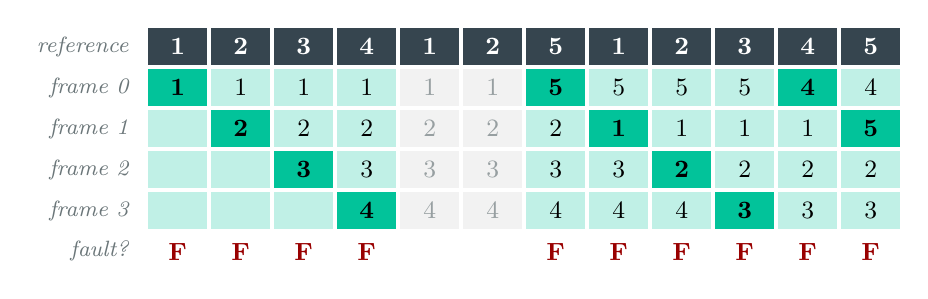
\begin{tikzpicture}[c/.style={rectangle,minimum width=0.75cm,minimum height=0.47cm,inner sep=0pt,font=\small}]
\node[anchor=east,font=\footnotesize\itshape,text=muted] at (-0.1,0.00) {reference};
\node[anchor=east,font=\footnotesize\itshape,text=muted] at (-0.1,-0.52) {frame 0};
\node[anchor=east,font=\footnotesize\itshape,text=muted] at (-0.1,-1.04) {frame 1};
\node[anchor=east,font=\footnotesize\itshape,text=muted] at (-0.1,-1.56) {frame 2};
\node[anchor=east,font=\footnotesize\itshape,text=muted] at (-0.1,-2.08) {frame 3};
\node[anchor=east,font=\footnotesize\itshape,text=muted] at (-0.1,-2.60) {fault?};
\node[c,fill=charcoal,text=white,font=\small\bfseries] at (0.40,0) {1};
\node[c,fill=mint,text=black] at (0.40,-0.52) {\bfseries1};
\node[c,fill=mint!25,text=black] at (0.40,-1.04) {};
\node[c,fill=mint!25,text=black] at (0.40,-1.56) {};
\node[c,fill=mint!25,text=black] at (0.40,-2.08) {};
\node[c,text=red!60!black,font=\small\bfseries] at (0.40,-2.60) {F};
\node[c,fill=charcoal,text=white,font=\small\bfseries] at (1.20,0) {2};
\node[c,fill=mint!25,text=black] at (1.20,-0.52) {1};
\node[c,fill=mint,text=black] at (1.20,-1.04) {\bfseries2};
\node[c,fill=mint!25,text=black] at (1.20,-1.56) {};
\node[c,fill=mint!25,text=black] at (1.20,-2.08) {};
\node[c,text=red!60!black,font=\small\bfseries] at (1.20,-2.60) {F};
\node[c,fill=charcoal,text=white,font=\small\bfseries] at (2.00,0) {3};
\node[c,fill=mint!25,text=black] at (2.00,-0.52) {1};
\node[c,fill=mint!25,text=black] at (2.00,-1.04) {2};
\node[c,fill=mint,text=black] at (2.00,-1.56) {\bfseries3};
\node[c,fill=mint!25,text=black] at (2.00,-2.08) {};
\node[c,text=red!60!black,font=\small\bfseries] at (2.00,-2.60) {F};
\node[c,fill=charcoal,text=white,font=\small\bfseries] at (2.80,0) {4};
\node[c,fill=mint!25,text=black] at (2.80,-0.52) {1};
\node[c,fill=mint!25,text=black] at (2.80,-1.04) {2};
\node[c,fill=mint!25,text=black] at (2.80,-1.56) {3};
\node[c,fill=mint,text=black] at (2.80,-2.08) {\bfseries4};
\node[c,text=red!60!black,font=\small\bfseries] at (2.80,-2.60) {F};
\node[c,fill=charcoal,text=white,font=\small\bfseries] at (3.60,0) {1};
\node[c,fill=light,text=muted!70] at (3.60,-0.52) {1};
\node[c,fill=light,text=muted!70] at (3.60,-1.04) {2};
\node[c,fill=light,text=muted!70] at (3.60,-1.56) {3};
\node[c,fill=light,text=muted!70] at (3.60,-2.08) {4};
\node[c,fill=charcoal,text=white,font=\small\bfseries] at (4.40,0) {2};
\node[c,fill=light,text=muted!70] at (4.40,-0.52) {1};
\node[c,fill=light,text=muted!70] at (4.40,-1.04) {2};
\node[c,fill=light,text=muted!70] at (4.40,-1.56) {3};
\node[c,fill=light,text=muted!70] at (4.40,-2.08) {4};
\node[c,fill=charcoal,text=white,font=\small\bfseries] at (5.20,0) {5};
\node[c,fill=mint,text=black] at (5.20,-0.52) {\bfseries5};
\node[c,fill=mint!25,text=black] at (5.20,-1.04) {2};
\node[c,fill=mint!25,text=black] at (5.20,-1.56) {3};
\node[c,fill=mint!25,text=black] at (5.20,-2.08) {4};
\node[c,text=red!60!black,font=\small\bfseries] at (5.20,-2.60) {F};
\node[c,fill=charcoal,text=white,font=\small\bfseries] at (6.00,0) {1};
\node[c,fill=mint!25,text=black] at (6.00,-0.52) {5};
\node[c,fill=mint,text=black] at (6.00,-1.04) {\bfseries1};
\node[c,fill=mint!25,text=black] at (6.00,-1.56) {3};
\node[c,fill=mint!25,text=black] at (6.00,-2.08) {4};
\node[c,text=red!60!black,font=\small\bfseries] at (6.00,-2.60) {F};
\node[c,fill=charcoal,text=white,font=\small\bfseries] at (6.80,0) {2};
\node[c,fill=mint!25,text=black] at (6.80,-0.52) {5};
\node[c,fill=mint!25,text=black] at (6.80,-1.04) {1};
\node[c,fill=mint,text=black] at (6.80,-1.56) {\bfseries2};
\node[c,fill=mint!25,text=black] at (6.80,-2.08) {4};
\node[c,text=red!60!black,font=\small\bfseries] at (6.80,-2.60) {F};
\node[c,fill=charcoal,text=white,font=\small\bfseries] at (7.60,0) {3};
\node[c,fill=mint!25,text=black] at (7.60,-0.52) {5};
\node[c,fill=mint!25,text=black] at (7.60,-1.04) {1};
\node[c,fill=mint!25,text=black] at (7.60,-1.56) {2};
\node[c,fill=mint,text=black] at (7.60,-2.08) {\bfseries3};
\node[c,text=red!60!black,font=\small\bfseries] at (7.60,-2.60) {F};
\node[c,fill=charcoal,text=white,font=\small\bfseries] at (8.40,0) {4};
\node[c,fill=mint,text=black] at (8.40,-0.52) {\bfseries4};
\node[c,fill=mint!25,text=black] at (8.40,-1.04) {1};
\node[c,fill=mint!25,text=black] at (8.40,-1.56) {2};
\node[c,fill=mint!25,text=black] at (8.40,-2.08) {3};
\node[c,text=red!60!black,font=\small\bfseries] at (8.40,-2.60) {F};
\node[c,fill=charcoal,text=white,font=\small\bfseries] at (9.20,0) {5};
\node[c,fill=mint!25,text=black] at (9.20,-0.52) {4};
\node[c,fill=mint,text=black] at (9.20,-1.04) {\bfseries5};
\node[c,fill=mint!25,text=black] at (9.20,-1.56) {2};
\node[c,fill=mint!25,text=black] at (9.20,-2.08) {3};
\node[c,text=red!60!black,font=\small\bfseries] at (9.20,-2.60) {F};
\end{tikzpicture}
\caption{FIFO on the same string: \textbf{9 faults with 3 frames} (top) but \textbf{10 faults with 4 frames} (bottom).}
\end{figure}

This is \term{Belady's anomaly}. LRU and OPT never show it. They belong to the class of \term{stack algorithms}: the set of pages in memory with $n$ frames is always a subset of the set with $n+1$ frames (for LRU: the $n$ most recently used pages are always among the $n+1$ most recently used). Adding a frame can therefore never add a fault. On the same string, LRU needs $10$ faults with $3$ frames and $8$ with $4$.

\begin{histnote}[László Bélády]
The Hungarian-born computer scientist László Bélády worked at IBM Research. In 1966 he published the optimal replacement algorithm (MIN), and in 1969, with R.\,A.\ Nelson and G.\,S.\ Shedler, the paper describing the anomaly that now carries his name.
\end{histnote}

\subsection{Approximating LRU: reference bit and the clock}
\label{sec:clock}

Many CPUs provide a \term{reference bit} for each page: the hardware sets it to $1$ whenever the page is read or written. The OS can read it and clear it to $0$. The bit does not say \emph{when} a page was used, but it does say whether it was used \emph{since the bit was last cleared}.

The \term{second-chance} or \term{clock} algorithm arranges the frames in a circle with a pointer, the ``clock hand'', at the next candidate:
\begin{itemize}
  \item If the page under the hand has $R = 1$, it gets a second chance: set $R = 0$ and advance the hand.
  \item If it has $R = 0$, it has not been used since the hand last passed: it is the victim.
\end{itemize}

\begin{figure}[H]
\centering
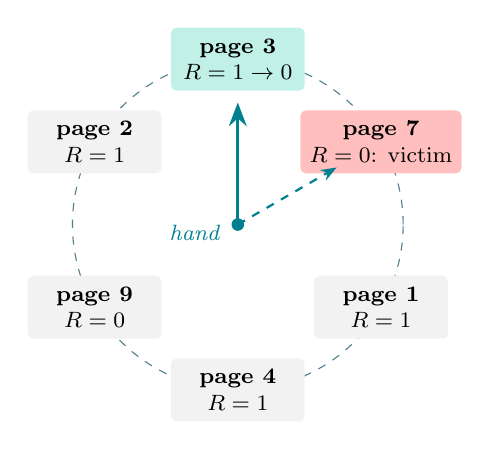
\begin{tikzpicture}[f/.style={rectangle,rounded corners=2pt,minimum width=1.7cm,minimum height=0.8cm,align=center,font=\footnotesize}]
\draw[dashed,slate] (0,0) circle (2.1);
\foreach \a/\p/\r/\c in {90/3/{$R=1\to0$}/mint!25,30/7/{$R=0$: victim}/red!25,-30/1/{$R=1$}/light,-90/4/{$R=1$}/light,-150/9/{$R=0$}/light,150/2/{$R=1$}/light}
  \node[f,fill=\c] at (\a:2.1) {\textbf{page \p}\\\r};
\fill[mintdeep] (0,0) circle (0.08);
\draw[-{Stealth[length=3mm]},very thick,mintdeep] (0,0) -- (90:1.55);
\draw[-{Stealth[length=2mm]},thick,mintdeep,dashed] (0,0) -- (30:1.45);
\node[font=\footnotesize\itshape,text=mintdeep] at (-0.55,-0.1) {hand};
\end{tikzpicture}
\caption{The hand is at page 3 ($R=1$): its bit is cleared and the hand moves on to page 7 ($R=0$), which is replaced.}
\end{figure}

If all bits are $1$, the hand goes once around the circle clearing them and the algorithm degenerates to FIFO. Real systems use refinements of this idea; Linux, for instance, keeps ``active'' and ``inactive'' page lists.

% =====================================================================
\section{Thrashing and the Working Set}

\subsection{Thrashing}

Suppose a process is actively using more pages than it has frames. It faults, and the page it evicts is one it needs again soon, so it faults again, and again. A process that spends more time paging than executing is \term{thrashing}.

\begin{figure}[H]
\centering
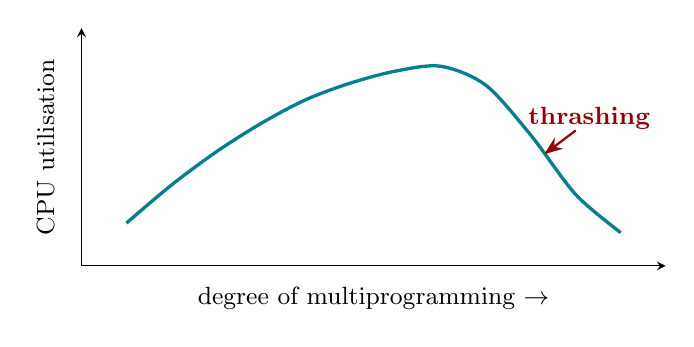
\begin{tikzpicture}
\begin{axis}[width=9cm,height=4.6cm,xmin=0,xmax=13,ymin=0,ymax=100,
  xlabel={degree of multiprogramming $\rightarrow$},ylabel={CPU utilisation},
  xtick=\empty,ytick=\empty,axis lines=left,
  every axis label/.style={font=\small},
  xlabel style={at={(axis description cs:0.5,-0.05)}},ylabel style={at={(axis description cs:-0.03,0.5)}}]
\addplot[very thick,mintdeep,smooth] coordinates {(1,18) (2,34) (3,48) (4,60) (5,70) (6,77) (7,82) (8,84) (9,76) (10,55) (11,30) (12,14)};
\node[font=\small\bfseries,text=red!60!black] at (axis cs:11.3,62) {thrashing};
\draw[-{Stealth},red!60!black,thick] (axis cs:11.0,57) -- (axis cs:10.3,47);
\end{axis}
\end{tikzpicture}
\caption{CPU utilisation against the number of processes in memory (conceptual curve, not measured data).}
\end{figure}

The curve explains the danger. Adding processes first raises CPU utilisation (more processes to run while others wait for I/O). Beyond some point the processes no longer have enough frames each; page faults explode, processes queue for the paging disk, and CPU utilisation collapses. A naive scheduler that reacts to the idle CPU by admitting even more processes makes things worse --- a vicious circle. The cure is to \emph{reduce} the degree of multiprogramming (suspend or swap out some processes) or to add physical memory. If you have ever used a computer with too little RAM and too many browser tabs, with the disk light constantly on and the mouse barely moving, you have seen thrashing.

\subsection{The working-set model}

The \term{working set} of a process at time $t$, $\text{WS}(t,\Delta)$, is the set of distinct pages referenced in its most recent $\Delta$ references; $\Delta$ is called the working-set window. The working set approximates the program's current locality.

\begin{figure}[H]
\centering
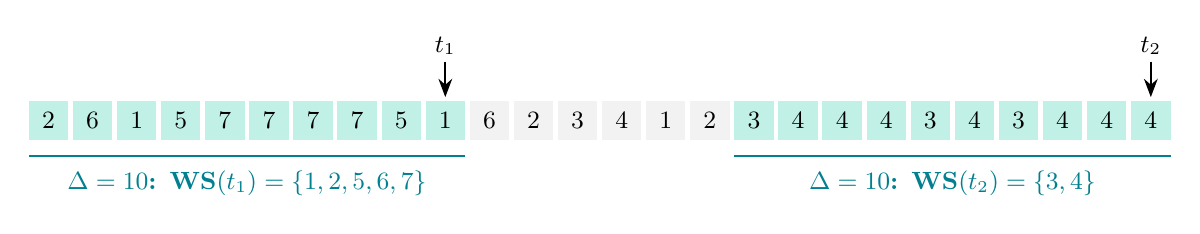
\begin{tikzpicture}[c/.style={rectangle,minimum width=0.5cm,minimum height=0.5cm,inner sep=0pt,font=\small}]
\foreach \v [count=\i from 0] in {2,6,1,5,7,7,7,7,5,1,6,2,3,4,1,2,3,4,4,4,3,4,3,4,4,4} {
  \pgfmathsetmacro{\inw}{(\i<=9)||(\i>=16)}
  \ifdim\inw pt>0pt \node[c,fill=mint!25] at (\i*0.56,0) {\v}; \else \node[c,fill=light] at (\i*0.56,0) {\v}; \fi
}
\draw[mintdeep,thick] (-0.25,-0.45) -- (5.29,-0.45);
\node[font=\small\bfseries,text=mintdeep] at (2.52,-0.8) {$\Delta=10$: $\text{WS}(t_1)=\{1,2,5,6,7\}$};
\draw[mintdeep,thick] (8.71,-0.45) -- (14.25,-0.45);
\node[font=\small\bfseries,text=mintdeep] at (11.48,-0.8) {$\Delta=10$: $\text{WS}(t_2)=\{3,4\}$};
\draw[-{Stealth},thick] (5.04,0.75) -- (5.04,0.3); \node[font=\small] at (5.04,0.95) {$t_1$};
\draw[-{Stealth},thick] (14.0,0.75) -- (14.0,0.3); \node[font=\small] at (14.0,0.95) {$t_2$};
\end{tikzpicture}
\caption{The working set follows the program's locality: 5 pages at $t_1$, only 2 at $t_2$.}
\end{figure}

If $\text{WSS}_i = |\text{WS}_i|$ is the working-set size of process $i$, the total demand for frames is $D = \sum_i \text{WSS}_i$. If $D$ exceeds the number of available frames $m$, thrashing will occur, and the OS should suspend a process until frames become available. The choice of $\Delta$ matters: too small and it misses part of the locality; too large and it overlaps several localities and wastes frames.

A simpler practical relative is \emph{page-fault frequency} control: the OS measures each process's fault rate, gives it more frames when the rate is too high, and takes frames away when it is very low.

% =====================================================================
\section{The File Concept}

Main memory is volatile and too small to keep everything. The OS therefore offers a second storage abstraction that survives power-off: the \term{file}, a named collection of related information recorded on secondary storage. From the user's point of view, a file is the smallest unit of storage that can be saved: you cannot write data to the disk except inside a file.

\Needspace{16\baselineskip}
\subsection{File attributes}

Besides its contents, every file has \term{attributes} (metadata). The right-hand column shows the values for a real file, taken from the \cmd{stat} output in Section~\ref{sec:links}.

\begin{center}
\renewcommand{\arraystretch}{1.3}
\begin{tabularx}{\linewidth}{>{\raggedright\arraybackslash}p{2.3cm} >{\raggedright\arraybackslash}X >{\raggedright\arraybackslash}p{4.4cm}}
\toprule
\textbf{Attribute} & \textbf{Meaning} & \textbf{Example (\texttt{notes.txt})} \\
\midrule
Name & Human-readable name; in Linux it is stored in the directory, not with the other attributes. & \texttt{notes.txt} \\
Identifier & Unique number of the file inside the file system. & inode $368662$ \\
Type & Regular file, directory, symbolic link, device, \dots & regular file \\
Location & Where the file's data blocks are on the device. & block pointers in the inode \\
Size & Current size in bytes (and blocks allocated). & $6$ bytes ($8$ blocks of $512$~B) \\
Protection & Who may read, write, execute. & \texttt{-rw-rw-r--}, owner \texttt{student} \\
Timestamps & Creation, last access, last modification, last status change. & Access / Modify / Change / Birth \\
\bottomrule
\end{tabularx}
\end{center}

The OS keeps these attributes in a per-file structure called the \term{file control block} (FCB). In UNIX and Linux the FCB is the \term{inode} (Section~\ref{sec:inode}).

\subsection{File operations}

A file is an \emph{abstract data type}: it is defined by the operations you can apply to it. The basic operations, with the corresponding Linux system calls, are:

\begin{center}
\renewcommand{\arraystretch}{1.25}
\begin{tabularx}{\linewidth}{>{\bfseries}l >{\raggedright\arraybackslash}X l}
\toprule
\textbf{Operation} & \textbf{What the OS does} & \textbf{Linux call} \\
\midrule
create & Find space in the file system and add an entry to the directory. & \cmd{open(\dots, O\_CREAT)} \\
open & Search the directory once, check permissions, return a \emph{file descriptor}. & \cmd{open()} \\
read & Copy bytes from the file, starting at the current position. & \cmd{read()} \\
write & Copy bytes into the file, starting at the current position. & \cmd{write()} \\
seek & Move the current position (``reposition''); no data is transferred. & \cmd{lseek()} \\
close & Release the open-file table entry. & \cmd{close()} \\
delete & Remove the directory entry; free the space when no longer used. & \cmd{unlink()} \\
truncate & Erase the contents but keep the attributes. & \cmd{truncate()} \\
\bottomrule
\end{tabularx}
\end{center}

Other operations (append, rename, copy) can be built from these. Note the name \cmd{unlink()} for delete: it removes one \emph{name} of the file; Section~\ref{sec:acyclic} explains why that is not always the same as deleting the data.

\subsection{The open-file tables}

Searching the directory and checking permissions for every single \cmd{read()} would be slow. Instead, \cmd{open()} does this work once and stores the result in memory tables; it returns a small integer, the \term{file descriptor}, which the process uses in all later calls. Descriptors $0$, $1$ and $2$ are already open when a program starts: standard input, standard output and standard error (Week~2).

\begin{figure}[H]
\centering
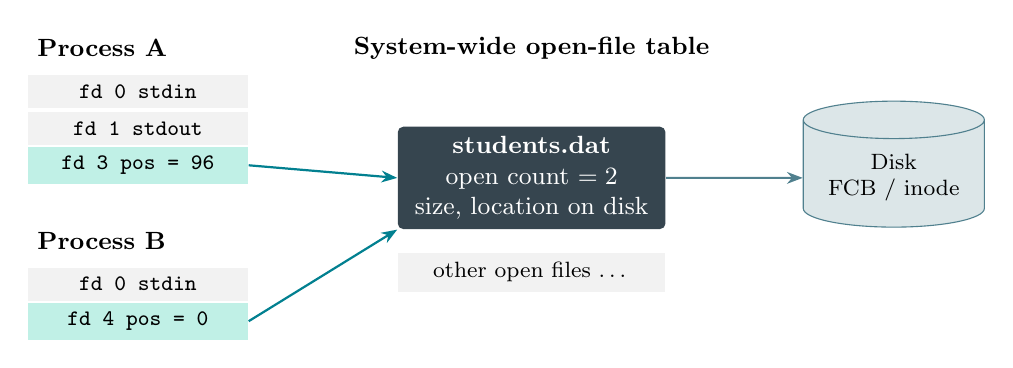
\begin{tikzpicture}[e/.style={rectangle,minimum width=2.8cm,minimum height=0.42cm,font=\footnotesize\ttfamily,fill=light},
  arr/.style={-{Stealth[length=2mm]},thick,mintdeep}]
\node[font=\small\bfseries,anchor=west] at (-1.4,0.55) {Process A};
\node[e] at (0,0) {fd 0  stdin}; \node[e] at (0,-0.47) {fd 1  stdout};
\node[e,fill=mint!25] (a3) at (0,-0.94) {fd 3  pos = 96};
\node[font=\small\bfseries,anchor=west] at (-1.4,-1.9) {Process B};
\node[e] at (0,-2.45) {fd 0  stdin};
\node[e,fill=mint!25] (b4) at (0,-2.92) {fd 4  pos = 0};
\node[font=\small\bfseries] at (5.0,0.55) {System-wide open-file table};
\node[rectangle,rounded corners=2pt,fill=charcoal,text=white,minimum width=3.4cm,minimum height=1.3cm,align=center,font=\small] (sw) at (5.0,-1.1) {\textbf{students.dat}\\open count $=2$\\size, location on disk};
\node[rectangle,fill=light,minimum width=3.4cm,minimum height=0.5cm,font=\footnotesize] at (5.0,-2.3) {other open files \dots};
\draw[arr] (a3.east) -- (sw.west);
\draw[arr] (b4.east) -- (sw.south west);
\node[cylinder,shape border rotate=90,aspect=0.25,draw=slate,fill=slate!20,minimum width=2.3cm,minimum height=1.6cm,align=center,font=\footnotesize] (dk) at (9.6,-1.1) {Disk\\FCB / inode};
\draw[arr,slate] (sw.east) -- (dk.west);
\end{tikzpicture}
\caption{Per-process tables hold each process's file pointer; the system-wide table holds shared information and an open count.}
\end{figure}

\begin{itemize}
  \item The \textbf{per-process open-file table} has one entry per open file of that process, with the \term{file pointer} (current position) and the access mode (read, write, \dots).
  \item The \textbf{system-wide open-file table} has one entry per open file, shared by all processes that have it open, with process-independent information: location on the disk, size, and an \term{open count}. \cmd{close()} decrements the count; when it reaches $0$ the entry is removed.
\end{itemize}
This is the textbook model. Linux adds one more level (descriptor $\to$ ``open file description'' holding the position $\to$ in-memory inode), but the idea is the same.

\subsection{File types and extensions}

The OS and applications must know what kind of data a file contains. The most common technique is to put the type into the name, as an \term{extension}:

\begin{center}
\renewcommand{\arraystretch}{1.25}
\begin{tabular}{@{}lll@{}}
\toprule
\textbf{File type} & \textbf{Usual extensions} & \textbf{Contents} \\
\midrule
Source code & \texttt{.c .py .java} & program text in a programming language \\
Object / executable & \texttt{.o .exe} (none on Linux) & machine code \\
Script & \texttt{.sh .bat} & commands for a command interpreter \\
Text / document & \texttt{.txt .pdf .docx} & text, formatted documents \\
Multimedia & \texttt{.jpg .mp3 .mp4} & image, sound, video \\
Archive & \texttt{.zip .tar.gz} & several files, often compressed \\
\bottomrule
\end{tabular}
\end{center}

Windows uses the extension to decide which program opens a file. In UNIX and Linux an extension is only a \emph{hint} for people and applications; the kernel does not care. The \cmd{file} command ignores the name and looks at the content, in particular at the first few bytes, which for many formats are a fixed \term{magic number} (an ELF executable starts with the bytes \texttt{7F 45 4C 46}, a JPEG image with \texttt{FF D8 FF}):

\Needspace{7\baselineskip}
\begin{lstlisting}[style=term]
$ file file_access.c
file_access.c: C source, ASCII text
$ file file_access
file_access: ELF 64-bit LSB pie executable, x86-64, version 1...
$ file photo.txt
photo.txt: JPEG image data, JFIF standard 1.01, aspect ratio,...
$ file students.dat
students.dat: data
\end{lstlisting}
Here \texttt{photo.txt} is really a JPEG picture with a misleading name, and \texttt{students.dat} is the binary record file written by Example~4 (long lines are cut with \texttt{...}).

% =====================================================================
\section{Access Methods}

How can the information in a file be read? The OS offers a few standard \term{access methods}.

\subsection{Sequential access}

Information is processed in order, one record after the other. A \emph{read next} returns the next portion of the file and advances the file pointer; \emph{write next} appends and advances; \emph{rewind} returns to the beginning. This is the model of a magnetic tape, and of most programs: editors, compilers and media players read their input from beginning to end.

\begin{figure}[H]
\centering
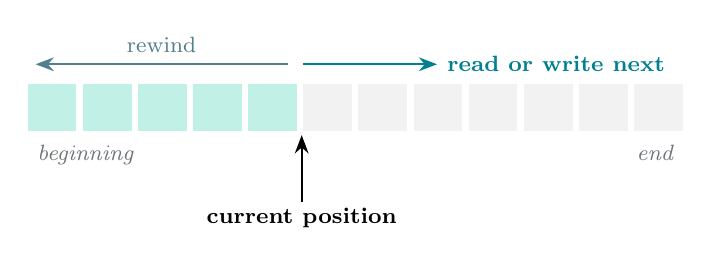
\begin{tikzpicture}
\foreach \i in {0,...,11} { \ifnum\i<5 \fill[mint!25] (\i*0.7,0) rectangle +(0.62,0.6); \else \fill[light] (\i*0.7,0) rectangle +(0.62,0.6); \fi }
\node[font=\footnotesize\itshape,text=muted,anchor=north west] at (0,-0.05) {beginning};
\node[font=\footnotesize\itshape,text=muted,anchor=north east] at (8.32,-0.05) {end};
\draw[-{Stealth},thick] (3.48,-0.9) -- (3.48,-0.05); \node[font=\footnotesize\bfseries] at (3.48,-1.1) {current position};
\draw[-{Stealth},thick,mintdeep] (3.5,0.85) -- (5.2,0.85) node[right,font=\footnotesize\bfseries] {read or write next};
\draw[-{Stealth},thick,slate] (3.3,0.85) -- (0.1,0.85); \node[font=\footnotesize,text=slate] at (1.7,1.1) {rewind};
\end{tikzpicture}
\caption{Sequential access.}
\end{figure}

\subsection{Direct (relative) access}

The file is viewed as a numbered sequence of fixed-size \emph{blocks} or \emph{records}, and any of them can be read or written in any order: \emph{read $n$}, \emph{write $n$}, or \emph{seek $n$} followed by read next. This matches a disk, which can reach any block in roughly the same time. Databases and reservation systems need direct access: to find seat 17C on a flight, you do not want to read all the seats before it.

The block number $n$ is \emph{relative} to the beginning of the file: block $0$, block $1$, and so on. The OS translates relative block numbers into physical disk blocks; the user never needs to know where on the device the file lies. Sequential access can easily be simulated on a direct-access file by keeping a current position $cp$: \emph{read next} means ``read block $cp$, then $cp \leftarrow cp+1$''.

\begin{example}[Where is record 1000?]
A file holds student records of $R = 100$ bytes each, numbered from $0$. The file system uses blocks of $B = 4096$ bytes. Which block holds record $k = 1000$, and where in the block does it start?
\begin{align*}
\text{byte offset} &= k \cdot R = 1000 \times 100 = 100\,000,\\
\text{block} &= \left\lfloor \frac{100\,000}{4096} \right\rfloor = 24,\\
\text{offset in block} &= 100\,000 - 24 \times 4096 = 100\,000 - 98\,304 = 1\,696 .
\end{align*}
The record's last byte is $100\,099$, and $\lfloor 100\,099 / 4096 \rfloor = 24$ as well, so the whole record lies in relative block $24$, bytes $1696$ to $1795$: one block read is enough. In C this is simply \cmd{lseek(fd, 1000 * 100, SEEK\_SET)} followed by \cmd{read(fd, rec, 100)}; the OS performs the division.
\end{example}

\subsection{Indexed access}

For large files, even direct access needs to know \emph{which} record number to read. An \term{index} solves this: a small, sorted file of (key, block number) pairs, for example student surnames with the block holding each student's record. To find a record, the OS or application searches the index (fast, because it is small and sorted) and then reads one block directly.


If the index itself becomes too large, it is indexed in turn (a multi-level index). This idea underlies database indexes such as B-trees, IBM's classic ISAM (indexed sequential access method), and the way file systems locate a file's own blocks.

\subsection{Hands-on: sequential and direct access in C}

Example 4 creates a file of five fixed-size $32$-byte records, reads them sequentially, jumps directly to record $3$ (byte $3 \times 32 = 96$) and overwrites record $1$ in place.

The listing shows the core of the program; the complete version, \cmd{file\_access.c}, also checks the return value of every call.

\lstinputlisting[caption={}]{../code/file_access_excerpt.c}

\Needspace{7\baselineskip}
\begin{lstlisting}[style=term]
$ ./file_access
sequential:  [0 Ayse]  [1 Mehmet]  [2 Elif]  [3 Can]  [4 Zeynep]
direct: record 3 at byte 96 -> [3 Can]
after update: record 1 -> [1 Mehmet (updated)]
file size: 160 bytes
\end{lstlisting}

The file pointer that \cmd{read()} advances and \cmd{lseek()} sets is exactly the ``current position'' kept in the per-process open-file table. The file is $5 \times 32 = 160$ bytes long; overwriting record $1$ did not change its size or touch the other records.

% =====================================================================
\section{Directory Structures}

A disk can hold millions of files. A \term{directory} (folder) is a symbol table that maps file names to their FCBs. Operations on directories include searching for a file, creating and deleting files, listing a directory, renaming, and traversing the whole file system (for backups, for example). How directories are organised has evolved through several stages.

\subsection{Single-level and two-level directories}

In a \term{single-level directory}, all files of all users are in one directory. It is simple, but every name must be unique: if two users both want a file called \texttt{test}, one of them loses. With hundreds of files, a single list becomes unmanageable.

A \term{two-level directory} gives each user a private \emph{user file directory} (UFD), listed in a \emph{master file directory} (MFD). Two users can now both have a file called \texttt{test}; a file is named by a path such as \texttt{/ayse/test}. Users are isolated from one another --- good for protection, but awkward when they want to share files, and there is still no way to group a user's own files.

\begin{figure}[H]
\centering
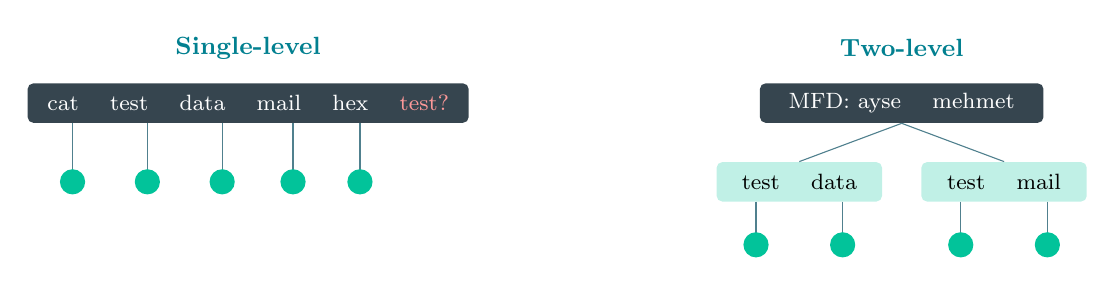
\begin{tikzpicture}[f/.style={circle,fill=mint,inner sep=0pt,minimum size=0.32cm},
  d/.style={rectangle,rounded corners=2pt,minimum height=0.5cm,font=\footnotesize}]
\begin{scope}
\node[font=\small\bfseries,text=mintdeep] at (2.4,1.0) {Single-level};
\node[d,fill=charcoal,text=white,minimum width=5.6cm] (sd) at (2.4,0.3) {cat \quad test \quad data \quad mail \quad hex \quad {\color{red!40}test?}};
\foreach \x in {0.05,1.0,1.95,2.85,3.7} { \draw[slate] (\x+0.12,0.05) -- (\x+0.12,-0.55); \node[f] at (\x+0.12,-0.7) {}; }
\end{scope}
\begin{scope}[xshift=8.3cm]
\node[font=\small\bfseries,text=mintdeep] at (2.4,1.0) {Two-level};
\node[d,fill=charcoal,text=white,minimum width=3.6cm] (m) at (2.4,0.3) {MFD: ayse \quad mehmet};
\node[d,fill=mint!25,minimum width=2.1cm] (u1) at (1.1,-0.7) {test \quad data};
\node[d,fill=mint!25,minimum width=2.1cm] (u2) at (3.7,-0.7) {test \quad mail};
\draw[slate] (m.south) -- (u1.north); \draw[slate] (m.south) -- (u2.north);
\foreach \x in {0.55,1.65,3.15,4.25} { \draw[slate] (\x,-0.95) -- (\x,-1.35); \node[f] at (\x,-1.5) {}; }
\end{scope}
\end{tikzpicture}
\caption{Single-level: one name space for everyone (the second \texttt{test} clashes). Two-level: one directory per user.}
\end{figure}

\subsection{Tree-structured directories}

The natural generalisation is a \term{tree}: a directory may contain files \emph{and} other directories (subdirectories), to any depth. Every modern operating system uses a tree, or one of the generalisations below. Each process has a \term{current working directory}.

\begin{figure}[H]
\centering
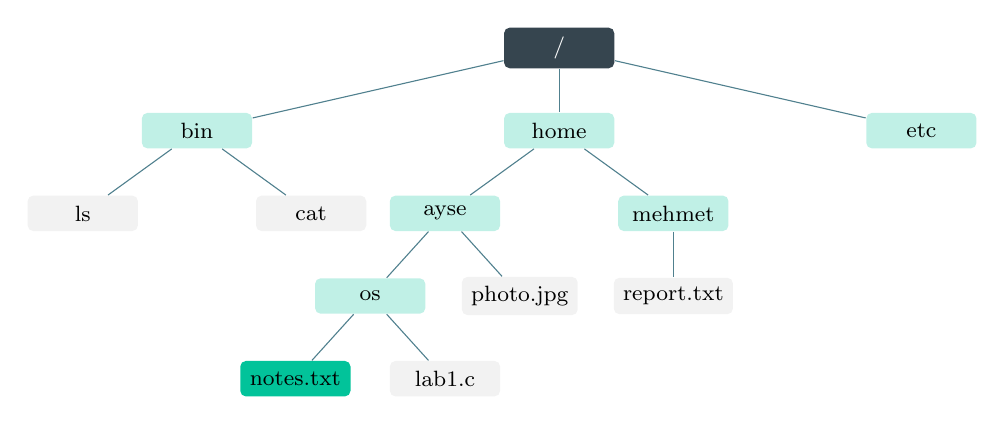
\begin{tikzpicture}[level distance=1.05cm,
  dir/.style={rectangle,rounded corners=2pt,fill=mint!25,minimum width=1.4cm,minimum height=0.45cm,font=\footnotesize},
  fil/.style={rectangle,rounded corners=2pt,fill=light,minimum width=1.4cm,minimum height=0.45cm,font=\footnotesize},
  level 1/.style={sibling distance=4.6cm}, level 2/.style={sibling distance=2.9cm}, level 3/.style={sibling distance=1.9cm},
  edge from parent/.style={draw,slate}]
\node[dir,fill=charcoal,text=white] {/}
  child {node[dir] {bin} child {node[fil] {ls}} child {node[fil] {cat}}}
  child {node[dir] {home}
     child {node[dir] {ayse} child {node[dir] {os} child {node[fil,fill=mint] {notes.txt}} child {node[fil] {lab1.c}}} child {node[fil] {photo.jpg}}}
     child {node[dir] {mehmet} child {node[fil] {report.txt}}}}
  child {node[dir] {etc}};
\end{tikzpicture}
\caption{A tree-structured directory (pale: directories; grey: files).}
\label{fig:tree}
\end{figure}

A file can be named in two ways:
\begin{itemize}
  \item \texttt{/home/ayse/os/notes.txt} is an \term{absolute path}: it starts at the root \texttt{/}, lists every directory on the way, and works from anywhere.
  \item A \term{relative path} starts at the current directory. If the current directory is \texttt{/home/ayse}, the same file is \texttt{os/notes.txt}.
\end{itemize}
Every directory contains two special entries: \texttt{.} (the directory itself) and \texttt{..} (its parent). From \texttt{/\allowbreak{}home/\allowbreak{}ayse/\allowbreak{}os}, Mehmet's report is \texttt{../\allowbreak{}../\allowbreak{}mehmet/\allowbreak{}report.txt}. In the shell, \texttt{\textasciitilde} is short for your home directory. Windows uses the same idea with drive letters and backslashes: \texttt{C:\textbackslash{}Users\textbackslash{}ayse\textbackslash{}os\textbackslash{}notes.txt}. In Week~9 you will move around this tree with \cmd{pwd}, \cmd{cd} and \cmd{ls}.

\subsection{Acyclic-graph directories: hard and symbolic links}
\label{sec:acyclic}

A tree cannot express \emph{sharing}: if Ayşe and Mehmet work on the same project, the project file should appear in both their directories --- not as two copies that drift apart, but as one file. An \term{acyclic-graph directory} allows a file or subdirectory to appear in several directories, as long as no cycles are formed. UNIX and Linux offer two kinds of \term{link}:

\begin{itemize}
  \item A \term{hard link} is a second directory entry pointing to the \emph{same} inode. Both names are equal; neither is ``the original''. The inode keeps a \term{link count}, the number of directory entries pointing to it. Deleting a name (\cmd{unlink}) decrements the count; the data is freed only when the count reaches $0$ and no process has the file open. Hard links cannot cross file systems and (in Linux) cannot point to directories.
  \item A \term{symbolic link} (soft link) is a small separate file whose content is a \emph{path name}. Opening it makes the OS follow the path. It can point to directories and across file systems, but if the target is deleted or moved, the link \emph{dangles}.
\end{itemize}

\begin{figure}[H]
\centering
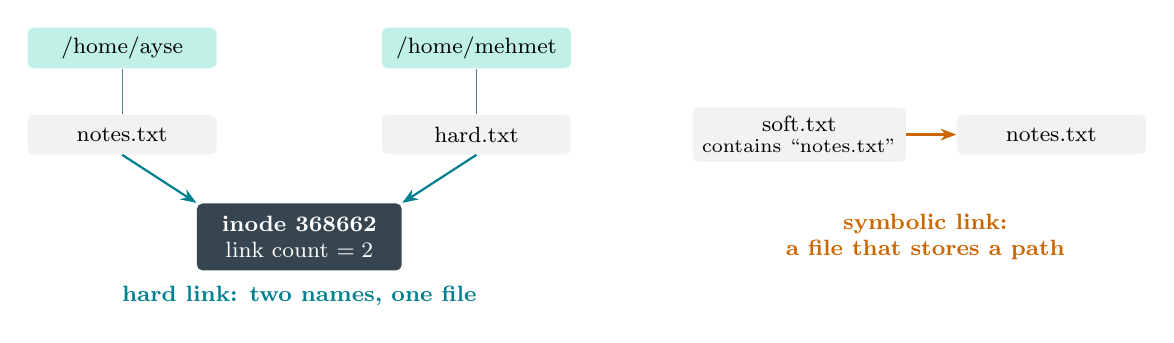
\begin{tikzpicture}[d/.style={rectangle,rounded corners=2pt,fill=mint!25,minimum width=2.4cm,minimum height=0.5cm,font=\footnotesize},
  n/.style={rectangle,rounded corners=2pt,fill=light,minimum width=2.4cm,minimum height=0.5cm,font=\footnotesize,align=center},
  arr/.style={-{Stealth[length=2mm]},thick,mintdeep}]
\node[d] (a) at (0,0) {/home/ayse}; \node[d] (m) at (4.5,0) {/home/mehmet};
\node[n] (nt) at (0,-1.1) {notes.txt}; \node[n] (ht) at (4.5,-1.1) {hard.txt};
\draw[slate] (a) -- (nt); \draw[slate] (m) -- (ht);
\node[rectangle,rounded corners=2pt,fill=charcoal,text=white,minimum width=2.6cm,minimum height=0.85cm,align=center,font=\footnotesize] (ino) at (2.25,-2.4) {\textbf{inode 368662}\\link count $=2$};
\draw[arr] (nt.south) -- (ino.north west); \draw[arr] (ht.south) -- (ino.north east);
\node[font=\footnotesize\bfseries,text=mintdeep] at (2.25,-3.15) {hard link: two names, one file};
\begin{scope}[xshift=8.6cm]
\node[n] (s) at (0,-1.1) {soft.txt\\[-2pt]{\scriptsize contains ``notes.txt''}};
\node[n] (t) at (3.2,-1.1) {notes.txt};
\draw[arr,orange!80!black] (s.east) -- (t.west);
\node[font=\footnotesize\bfseries,text=orange!80!black,align=center] at (1.6,-2.4) {symbolic link:\\a file that stores a path};
\end{scope}
\end{tikzpicture}
\caption{A hard link is another name for the same inode; a symbolic link is a file containing a path.}
\end{figure}

\subsection{General-graph directories}

If links are allowed to point to \emph{any} directory, including an ancestor, the directory structure can contain \term{cycles}. Two problems appear: a program that walks the file system (search, backup) may loop forever, and a subtree that has been ``deleted'' may still be referenced from within itself, so its link count never drops to $0$ and its space is never freed without expensive garbage collection. Practical systems avoid general graphs: Linux forbids hard links to directories, and when a chain of symbolic links loops, path lookup stops with the error \texttt{ELOOP} (``too many levels of symbolic links'').

% =====================================================================
\section{What Linux Shows: Inodes and Links}
\label{sec:inode}

In Linux, a directory is just a table of (name, inode number) pairs. Everything else about a file --- type, permissions, owner, size, timestamps, link count and the pointers to its data blocks --- is stored in its \term{inode}. The inode does \emph{not} contain the file's name; that is why one inode can have several names.

\begin{figure}[H]
\centering
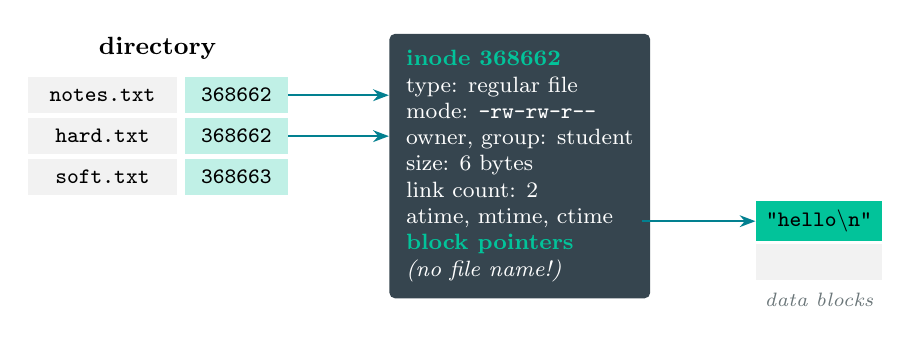
\begin{tikzpicture}[e/.style={rectangle,fill=light,minimum height=0.45cm,font=\footnotesize\ttfamily},
  arr/.style={-{Stealth[length=2mm]},thick,mintdeep}]
\node[font=\small\bfseries] at (1.4,0.6) {directory};
\foreach \n/\i [count=\k from 0] in {notes.txt/368662,hard.txt/368662,soft.txt/368663} {
  \node[e,minimum width=1.9cm] at (0.7,-0.52*\k) {\n};
  \node[e,minimum width=1.3cm,fill=mint!25] (d\k) at (2.4,-0.52*\k) {\i};
}
\node[rectangle,rounded corners=2pt,fill=charcoal,text=white,align=left,font=\footnotesize,inner sep=6pt] (ino) at (6.0,-0.9) {\textbf{\color{mint}inode 368662}\\type: regular file\\mode: \texttt{-rw-rw-r--}\\owner, group: student\\size: 6 bytes\\link count: 2\\atime, mtime, ctime\\\textbf{\color{mint}block pointers}\\{\itshape\color{white!60}(no file name!)}};
\draw[arr] (d0.east) -- (ino.west |- d0); \draw[arr] (d1.east) -- (ino.west |- d1);
\node[rectangle,fill=mint,minimum width=1.6cm,minimum height=0.45cm,font=\footnotesize\ttfamily] (db) at (9.8,-1.6) {"hello\textbackslash n"};
\node[rectangle,fill=light,minimum width=1.6cm,minimum height=0.45cm] at (9.8,-2.12) {};
\node[font=\scriptsize\itshape,text=muted] at (9.8,-2.6) {data blocks};
\draw[arr] (7.55,-1.6) -- (db.west);
\end{tikzpicture}
\caption{Directory entries point to inodes; inodes point to data blocks.}
\end{figure}

Useful commands: \cmd{ls -i} prints inode numbers, the second column of \cmd{ls -l} is the link count, \cmd{stat} shows the whole inode, and \cmd{df -i} shows how many inodes are free. A consequence worth knowing: \cmd{mv} within one file system only changes directory entries, so moving even a huge file is instant --- the inode and data stay where they are.

\subsection{Hands-on: \texttt{ls -li}, \texttt{ln}, \texttt{ln -s} and \texttt{stat}}
\label{sec:links}

The script \cmd{code/links\_demo.sh} runs the following commands (better: type them one by one in an empty directory). Output captured as an ordinary user on our test machine:

\Needspace{7\baselineskip}
\begin{lstlisting}[style=term]
$ echo "hello" > notes.txt
$ ls -li notes.txt
368662 -rw-rw-r-- 1 student student 6 Oct  8 12:20 notes.txt
$ ln notes.txt hard.txt
$ ln -s notes.txt soft.txt
$ ls -li
total 8
368662 -rw-rw-r-- 2 student student 6 Oct  8 12:20 hard.txt
368662 -rw-rw-r-- 2 student student 6 Oct  8 12:20 notes.txt
368663 lrwxrwxrwx 1 student student 9 Oct  8 12:20 soft.txt -> notes.txt
$ stat notes.txt
  File: notes.txt
  Size: 6            Blocks: 8          IO Block: 4096   regular file
Device: 254,0   Inode: 368662      Links: 2
Access: (0664/-rw-rw-r--)  Uid: ( 1001/ student)   Gid: ( 1002/ student)
Access: 2026-10-08 12:20:48.530146698 +0000
Modify: 2026-10-08 12:20:48.530146698 +0000
Change: 2026-10-08 12:20:48.534146698 +0000
 Birth: 2026-10-08 12:20:48.530146698 +0000
$ rm notes.txt
$ cat hard.txt
hello
$ cat soft.txt
cat: soft.txt: No such file or directory
$ ls -li
total 4
368662 -rw-rw-r-- 1 student student 6 Oct  8 12:20 hard.txt
368663 lrwxrwxrwx 1 student student 9 Oct  8 12:20 soft.txt -> notes.txt
\end{lstlisting}

What to observe:
\begin{itemize}
  \item \texttt{notes.txt} and \texttt{hard.txt} have the \emph{same} inode number ($368662$) and a link count of $2$: two names, one file.
  \item \texttt{soft.txt} has its own inode ($368663$), type \texttt{l}, and size $9$: exactly the length of the string \texttt{notes.txt} it stores.
  \item In \cmd{stat}, \emph{Change} (ctime, the last change of the \emph{inode}) is a few milliseconds later than \emph{Modify} (mtime, the last change of the \emph{data}): creating the hard link updated the link count in the inode, not the contents.
  \item After \cmd{rm notes.txt}, the data is still reachable through \texttt{hard.txt} (link count back to $1$), while \texttt{soft.txt} dangles: the path it stores no longer exists.
\end{itemize}
This session is a preview of Week~10 (file operations: \cmd{cp}, \cmd{mv}, \cmd{rm}, \cmd{ln}) and Week~11, where the permission string \texttt{-rw-rw-r--}, stored in the inode, is explained in detail.

% =====================================================================
\section{Summary}

\begin{keyidea}[Week 7 in eight sentences]
\begin{enumerate}[leftmargin=1.4em]
  \item Virtual memory gives each process a large address space of which only the pages in use are in RAM; locality makes this work.
  \item Demand paging loads a page on its first use; the valid--invalid bit tells the MMU whether a page is in memory.
  \item An access to an invalid page traps to the OS (page fault), which loads the page and restarts the instruction; $\text{EAT} = (1-p)t_m + p\,t_{\text{fault}}$, so $p$ must be tiny.
  \item Copy-on-write shares pages after \cmd{fork()} until one process writes.
  \item When no frame is free, a replacement algorithm picks a victim: FIFO (15 faults in our example, Belady's anomaly possible), OPT (9, optimal but needs the future), LRU (12, approximated by the clock algorithm).
  \item Thrashing occurs when processes have fewer frames than their working sets; the cure is fewer processes in memory.
  \item A file is a named collection of data with attributes; it is opened once and then accessed sequentially, directly (block arithmetic) or through an index.
  \item Directories evolved from single-level to two-level to trees and acyclic graphs; in Linux, directory entries map names to inodes, and hard and symbolic links give a file several names.
\end{enumerate}
\end{keyidea}

% =====================================================================
\Needspace{12\baselineskip}
\section{Glossary}

\begin{description}[leftmargin=0pt,itemsep=0.15em]
  \item[Backing store] Disk area that holds the pages of processes that are not in RAM (swap space).
  \item[Belady's anomaly] More frames causing more page faults; possible with FIFO.
  \item[Clock (second-chance) algorithm] LRU approximation that scans frames in a circle using the reference bit.
  \item[Dirty (modify) bit] Hardware bit set when a page is written; clean pages need not be written back.
  \item[File control block / inode] Per-file structure holding a file's attributes and block locations.
  \item[Hard link] An additional directory entry for an existing inode.
  \item[Page fault] Trap raised when a process accesses a page that is not in memory.
  \item[Symbolic link] A file whose content is the path of another file.
  \item[Thrashing] State in which processes spend more time paging than executing.
  \item[Valid--invalid bit] Page-table bit that tells whether a page is in memory.
  \item[Virtual memory] Separation of a program's address space from physical memory, allowing it to be larger than RAM.
  \item[Working set] Set of distinct pages referenced in the last $\Delta$ references.
\end{description}

% =====================================================================
\Needspace{20\baselineskip}
\section{Try It Yourself}

\begin{tryit}[Page faults, page replacement and links on your own machine]
\textbf{Linux} (lab PCs, WSL, or a virtual machine), in the \texttt{code/} folder:
\Needspace{7\baselineskip}
\begin{lstlisting}[style=term]
$ make                          # builds the three C programs
$ ./page_faults                 # change 64 to 256 MB: what happens?
$ /usr/bin/time -v ./cow_fork   # look for "Minor ... page faults"
$ python3 page_replacement.py   # edit refs and frames, rerun
$ mkdir lab && cd lab && bash ../links_demo.sh
\end{lstlisting}
\begin{enumerate}[leftmargin=1.4em]
  \item In \cmd{page\_faults.c}, touch only every \emph{second} page in the first loop. How many faults do you expect, and how many do you get?
  \item Change the reference string in \cmd{page\_replacement.py} to one of your own and verify your hand-drawn FIFO, OPT and LRU tables.
  \item Make a hard link to a file, edit the file through one name and look at it through the other. Then try \cmd{ln} on a directory: what error do you get?
  \item Run \cmd{ls -li /} and \cmd{stat /}. Which inode number does the root directory have on your system?
\end{enumerate}
\end{tryit}

% =====================================================================
\section{Review Questions}

\subsection*{Conceptual}
\begin{enumerate}[leftmargin=1.6em]
  \item What is virtual memory, and why can a program run when only some of its pages are in RAM?
  \item Explain the difference between eager loading and demand paging. What is the price of demand paging?
  \item What does the valid--invalid bit mean? Give two different reasons for a page to be marked i.
  \item List the six steps of page-fault handling. Why must the faulting instruction be restarted?
  \item Explain copy-on-write. Why does it make \cmd{fork()} followed by \cmd{exec()} cheap?
  \item Why is OPT not implementable? Why is it still useful?
  \item What is Belady's anomaly? Which of FIFO, OPT and LRU can suffer from it?
  \item Describe thrashing and the vicious circle that can cause it. How does the working-set model help?
  \item Compare sequential, direct and indexed access, with one application for each.
  \item Compare hard and symbolic links: what happens to each when the original name is deleted?
\end{enumerate}

\subsection*{Numerical}
\begin{enumerate}[leftmargin=1.6em,resume]
  \item With $t_m = 200$~ns and $t_{\text{fault}} = 8$~ms, compute the EAT for $p = 0.0001$.
  \item With $t_m = 100$~ns and $t_{\text{fault}} = 5$~ms, what is the largest $p$ that keeps the slow-down below $20\%$?
  \item For the reference string $1, 2, 3, 1, 4, 1, 2$ with $3$ frames, count the page faults for FIFO, LRU and OPT.
  \item For the reference string $7, 0, 1, 2, 0, 3, 0, 4$ with $4$ frames, count the faults for FIFO and LRU.
  \item Records are $64$ bytes, blocks $4096$ bytes. In which relative block, and at which offset, does record $200$ start?
  \item A file has $250$-byte records and $1024$-byte blocks. Does record $40$ fit in a single block?
\end{enumerate}

\subsection*{Answers to the numerical questions}
\begin{enumerate}[leftmargin=1.6em,start=11]
  \item $\text{EAT} = 0.9999 \times 200 + 0.0001 \times 8\,000\,000 = 199.98 + 800 = 999.98\ \text{ns} \approx 1\ \mu\text{s}$, five times slower than RAM.
  \item Need $100 + p\,(5\,000\,000 - 100) < 120$, so $p < 20/4\,999\,900 \approx 4.0\times10^{-6}$: at most one fault per $250\,000$ accesses.
  \item FIFO: $1,2,3$ (3 faults), $1$ hit, $4$ replaces $1$, $1$ replaces $2$, $2$ replaces $3$: $6$ faults. LRU: $4$ replaces $2$ (least recently used), $1$ hit, $2$ replaces $3$: $5$ faults. OPT: $4$ replaces $3$ (never used again): $4$ faults.
  \item With $4$ frames, $7,0,1,2$ cause $4$ compulsory faults, $0$ is a hit, $3$ is a fault and so is $4$. FIFO: $3$ replaces $7$, $0$ hit, $4$ replaces $0$: $6$ faults. LRU: $3$ replaces $7$, $0$ hit, $4$ replaces $1$: $6$ faults.
  \item Offset $200 \times 64 = 12\,800$; block $\lfloor 12\,800/4096 \rfloor = 3$; offset in block $12\,800 - 3\times 4096 = 512$.
  \item Record $40$ occupies bytes $40 \times 250 = 10\,000$ to $10\,249$. $\lfloor 10\,000/1024 \rfloor = 9$ but $\lfloor 10\,249/1024 \rfloor = 10$: the record crosses a block boundary, so reading it needs two blocks.
\end{enumerate}

% =====================================================================
\section{Midterm Review: Weeks 1--7}

The midterm exam in Week~8 covers everything from Week~1 to this week. Use this list as a checklist; each item appeared in the slides and the course notes of the week shown.

\begin{description}[leftmargin=0pt,itemsep=0.2em]
  \item[Week 1: History] What an OS does; batch systems, multiprogramming, time-sharing; why idle CPUs drove OS design; UNIX (1969) and Linux (1991).
  \item[Week 2: OS basics] Definitions and the kernel; extended machine vs.\ resource manager; goals; interrupts; storage hierarchy; dual mode; system calls (\cmd{strace}); simple, monolithic, layered, microkernel, modular, hybrid structures.
  \item[Week 3: Processes] OS services; types of system calls; the process and its memory layout; process states; PCB; context switch; \cmd{fork()}.
  \item[Week 4: Threads, CPU] Threads vs.\ processes; user and kernel threads; multithreading models; CPU--I/O bursts; scheduling criteria (utilisation, throughput, turnaround, waiting and response time).
  \item[Week 5: Scheduling, sync] FCFS, SJF/SRTF, Priority, Round Robin with Gantt charts and average waiting time; race conditions; the critical-section problem; mutex locks; semaphores.
  \item[Week 6: Memory] Address binding; logical vs.\ physical addresses; MMU; swapping; contiguous allocation; internal and external fragmentation; paging and address translation; TLB and EAT; segmentation.
  \item[Week 7: VM, files] Demand paging; page faults; EAT with page faults; copy-on-write; FIFO, OPT, LRU tables; Belady's anomaly; clock; thrashing and working set; file attributes and operations; access methods with block arithmetic; directory structures; hard and symbolic links.
\end{description}

\textbf{Numerical question types to practise:} Gantt charts and waiting times (Week~5); address translation and EAT with a TLB (Week~6); EAT with page faults and page-replacement frame tables (Week~7); direct-access block arithmetic (Week~7). The best practice material is the set of review questions with worked answers at the end of each week's notes.

% =====================================================================
\section{Looking Ahead: Week 8 and Beyond}

\begin{itemize}
  \item \textbf{Week 8: Midterm exam} on Weeks~1--7. Bring your student ID and pens; the exact time, room and rules (for example about calculators) will be announced on the course Telegram channel.
  \item \textbf{Week 9} starts the hands-on half of the course: the Linux shell and navigating the directory tree we drew this week (\cmd{pwd}, \cmd{cd}, \cmd{ls}, absolute and relative paths).
  \item \textbf{Week 10:} file operations (\cmd{cp}, \cmd{mv}, \cmd{rm}, \cmd{ln}, \cmd{touch}); \textbf{Week 11:} permissions (the \texttt{-rw-rw-r--} string in the inode).
\end{itemize}

\subsection*{Further reading (optional)}
\begin{itemize}
  \item A.\ Silberschatz, P.\,B.\ Galvin and G.\ Gagne, \emph{Operating System Concepts}, 10th ed., Wiley: Chapter~10 (Virtual Memory), Chapter~13 (File-System Interface) and Section~14.1 (File-System Structure).
  \item R.\,H.\ and A.\,C.\ Arpaci-Dusseau, \emph{Operating Systems: Three Easy Pieces}:
  \begin{itemize}
    \item Chapter~21, ``Beyond Physical Memory: Mechanisms'': \url{https://pages.cs.wisc.edu/~remzi/OSTEP/vm-beyondphys.pdf}
    \item Chapter~22, ``Beyond Physical Memory: Policies'': \url{https://pages.cs.wisc.edu/~remzi/OSTEP/vm-beyondphys-policy.pdf}
    \item Chapter~39, ``Interlude: Files and Directories'': \url{https://pages.cs.wisc.edu/~remzi/OSTEP/file-intro.pdf}
  \end{itemize}
  \item L.\,A.\ Bélády, R.\,A.\ Nelson and G.\,S.\ Shedler, ``An anomaly in space-time characteristics of certain programs running in a paging machine'', \emph{Communications of the ACM} 12(6), 1969, pp.~349--353.
\end{itemize}

\end{document}
